\setchapterpreamble[u]{\margintoc}
\chapter{Existential Graphs}
\labch{eg}

\epigraph{

The System of Existential Graphs which I have now sufficiently described --- or,
at any rate, have described as well as I know how, leaving the further
perfection of it to others --- greatly facilitates the solution of problems of
Logic, as will be seen in the sequel, not by any mysterious properties, but
simply by substituting for the symbols in which such problems present
themselves, concrete visual figures concerning which we have merely to say
whether or not they admit certain describable relations of their parts.
Diagrammatic reasoning is the only really fertile reasoning. If logicians would
only embrace this method, we should no longer see attempts to base their science
on the fragile foundations of metaphysics or a psychology not based on logical
theory; and there would soon be such an advance in logic that every science
would feel the benefit of it.

}{\textbf{Charles S. Peirce}, \textit{Prolegomena to an Apology for
Pragmaticism}, 1906}


C. S. Peirce is famous for his contributions to symbolic logic, including among
others his eponymous law for classical logic, and his pioneering work on the
algebra of relations and quantification \cite{peirce_algebra_1885}. But far less
widespread are his achievements in the realm of graphical logic, or \emph{iconic
logic} as Shin calls it \cite{10.7551/mitpress/3633.001.0001}. He dedicated a
large chunk of his life investigating diagrammatic systems, starting in 1882
with the \emph{entitative graphs} and culminating with the \emph{existential
graphs}, which he developed from 1896 until his death in 1914
\cite{Roberts+1973}. Interestingly, Peirce perceived existential graphs
(thereafter ``EG'') as his \textit{``chef d'oeuvre''}, and that they
\textit{``ought to be the logic of the future''}\sidenote[][3em]{Both citations
are sourced in page 11 of \cite{Roberts+1973}.}.

Recent works have started to realize this vision: for example Sowa based his
conceptual graphs for computerized knowledge representation on EG
\cite{sowa_conceptual_1976}, Brady, Trimble
\cite{brady_categorical_2000}\cite{brady_string_nodate} and Haydon, Sobociński
\cite{pietarinen_compositional_2020} proposed various reconstructions of EG
through the lens of \emph{topology} and \emph{category theory}, and Melliès and
Zeilberger \cite{mellies_bifibrational_2016} refined the interpretation of Brady
and Trimble by making further connections with \emph{linear logic}
\cite{girard-linear-1987}. The full story has yet to be told, but we hope that
our work will constitute one more step towards the vision Peirce had in mind.

In this chapter, we propose a self-contained exposition of EG, that tries at the
same time to be faithful to the original presentation of the systems by Peirce,
and more modern in some aspects of their formalization. The goal will be to
familiarize the reader with the unique approach to proofs inherent to EG, which
can be difficult to relate to more standard frameworks like Hilbert and Gentzen
proof systems, and even deep inference proof systems like the calculus of
structures. This shall prove useful to get a good understanding of the
historical and technical foundations behind our \emph{flower calculus}, to be
introduced in \refch{flowers}.

The chapter is organized as follows: we start in \refsec{alpha} by presenting
the diagrammatic syntax of the system \sys{Alpha} of EG for classical
propositional logic. In \refsec{illative}, we introduce the inference rules of
\sys{Alpha} for manipulating existential graphs, called \emph{illative
transformations} by Peirce. In \refsec{multisets}, we give an equivalent
formulation of the syntax and rules of \sys{Alpha} as a \emph{multiset}
rewriting system. In \refsec{atomicity}, we formalize a variant of the
(de)iteration principle described by Peirce in
\sidecite{peirce_prolegomena_1906} that eliminates the need for the double-cut
principle, and discuss how it was motivated by Peirce's quest for \emph{illative
atomicity}. In \refsec{eg-soundness}, we take advantage of our reformulation to
give a simple proof of soundness for \sys{Alpha}, based on a direct
truth-evaluation of graphs. In \refsec{eg-completeness} we give a novel
syntactic proof of completeness for \sys{Alpha}, by simulating the calculus of
structures \sys{SKS} of Brünnler and Tiu \cite{brunnler_local_2001}. In this
way, \sys{Alpha} is shown to have subsystems that inherit the \emph{locality}
property of \sys{SKS}, and where the deletion and insertion rules are
respectively admissible for \emph{provability} and \emph{refutability}, making
\sys{Alpha} \emph{analytic}. In \refsec{beta}, we illustrate the original
mechanism of \emph{lines of identity} used by Peirce to handle quantifiers and
equality in his \sys{Beta} system. We end in \refsec{gardens} by showing how to
recast lines of identity in a more traditional binder-based syntax.

% \todo{IDEA (where should we put it?): \emph{superposition of polarities} in
% existential graphs. While a cut in bubble calculi is the insertion of \emph{two}
% occurrences of the same formula with \emph{distinct} polarities, the insertion
% rule only introduces \emph{one} occurrence of the formula, which plays either a
% negative role when it is iterated, or a positive role when it is deiterated}


\section{\sys{Alpha} graphs}\labsec{alpha}

Peirce designed in total three systems of EG, which he called respectively
\sys{Alpha}, \sys{Beta} and \sys{Gamma}. They were invented chronologically in
that order, which also captures their relationship in terms of complexity:
\sys{Alpha} is the foundation on which the other systems are built, and can
today be understood as a diagrammatic calculus for classical
\emph{propositional} logic. As we will see in \refsec{Quantification},
\sys{Beta} corresponds to a variable-free representation of \emph{predicate}
logic without function symbols, and with primitive support for \emph{equality}.
The last system \sys{Gamma} is more experimental, with various unfinished
features that have been interpreted as attempts to capture \emph{modal}
\sidecite{zeman_graphical_1964} and \emph{higher-order} logics\sidenote{A less
known fact is that at the end of his life, Peirce pushed his experimentations
beyond the scope of \emph{logic} in the contemporary sense of the word, with
so-called \emph{tinctured existential graphs} (Chapter 6 in
\cite{Roberts+1973}). Roughly, the idea was to represent a variety of
\emph{modes of expression} with different background shades on the canvas where
sentences are scribed, not unlike our graphical depiction of the \emph{status}
of solutions in \reffig{graphical-B}. In addition to the usual act of asserting
the truth of a proposition, one could for instance express a \emph{subjective}
or \emph{objective} possibility, or signify an interrogative or imperative mood,
all by using different colors. For print in publications, he would in fact use
\emph{heraldic tinctures} instead of colors, hence the ``tinctured''
qualificative. The precise meaning and purpose of tinctured EG remains elusive
to this day, and might constitute the most esoteric part of his work.}.
% We see a possible connection with the type-theoretical concept of
% \emph{judgment}, which was rehabilitated by Martin-Löf from the philosophy of
% Kant \cite{Martin-Lof1996-MAROTM-7}, who was of great influence on Peirce's own
% philosophy \cite{sep-peirce}.}.

The most fundamental concept of \sys{Alpha} is the \emph{sheet of assertion},
denoted by $\SA$ thereafter. It is the space where statements are scribed by the
reasoner, typically a sheet of paper or a blackboard. In a proof assistant, this
would either be the buffer of a text editor holding the theory the user is
developing, or the proof view displaying goals to be proved, depending on who
the reasoner is (the user or the computer, respectively). This last analogy
suggests an important property of $\SA$: it must offer a \emph{virtually
infinite} amount of space, so that one can perform as much reasoning as needed.
Just like a Turing machine has an infinite tape, so that one can perform as much
computation as needed. In symbolic logic, this is captured by the fact that
formulas, although usually finite, can have an unbounded size.

As its name indicates, scribing a statement on $\SA$ amounts to \emph{asserting
its truth}. Thus very naturally, the empty $\SA$ where nothing is scribed will
denote vacuous truth, traditionally symbolized by the formula
$\top$.

% \begin{remark}
%   Peirce had an \emph{externalist} conception of truth, where the assertions
% made by the \process{Graphist}, i.e. the person scribing on $\SA$, refer to the
% world \emph{outside} of the sheet (the universe of discourse). By not scribing
% anything, the \process{Graphist} thus refrains from asserting anything about the
% world, only assuming implicit truths. This is illustrated by the following
% quote, reminiscent of an interaction between a proof assistant (the
% \process{Graphist}) and its user (\process{the Interpreter})
% \cite[p.~92]{Roberts+1973}: \textit{``One of the parties, called the Graphist,
% is responsible for scribing the original graphs at the beginning of the
% investigation or discussion; the other, called the Interpreter, draws inferences
% from these graphs by changing them in accordance with the permissions of the
% system. The [...] sheet, before anything is scribed on it, represents whatever
% is taken for granted at the outset by the Graphist and Interpreter''}.
% \end{remark}

As we know from natural deduction, asserting the truth of the conjunction $a
\land b$ of two propositions $a$ and $b$, amounts to asserting \emph{both} the
truth of $a$ and the truth of $b$. In \sys{Alpha}, there is no need to introduce
the symbolic connective $\land$, since one can just write both $a$ and $b$ at
distinct locations on $\SA$:
$$a~~~b$$
More generally, one might consider any two portions $G$ and $H$ of $\SA$, and
interpret their \emph{juxtaposition} $G~H$ as signifying that we assert the
truth of their conjunction. This leads us to formulate the first fundamental
principle of \sys{Alpha}:
$$\text{\emph{Any portion of $\SA$ is a graph.}}$$
In particular, the entire $\SA$ itself is a graph.

Asserting the truth of the negation $\neg a$ of a proposition $a$, amounts to
\emph{denying} the truth of $a$. Using the original notation of Peirce, this is
done in \sys{Alpha} by \emph{enclosing} $a$ in a closed curve like so:
$$\pcut{a}$$ Peirce called such curves \emph{cuts}\sidenote{Not to be confused
with the name given to instances of the \emph{cut rule} in sequent calculus.
Although there is a connection, since in the one-sided version of \sys{LK}, one
occurrence of the cut formula in the premisses of the rule is negated.}, because
they ought to be seen as literal cuts in the paper sheet that embodies $\SA$.
Note that they do not need to be circles: all that matters is that $a$ is in a
separate area from the rest of $\SA$. This is precisely the content of the
\emph{Jordan curve theorem} in topology, and thus we can take cuts to be
arbitrary Jordan curves. This entails in particular that cuts cannot intersect
each other, but can be freely nested inside each other. Then as for
juxtaposition, one can replace $a$ by any graph $G$, i.e. any portion of $\SA$,
as long as the cut does not intersect other cuts in $G$.

With just these two \emph{icons}, juxtaposition and cuts, one can therefore
assert the truth of any proposition made up of conjunctions and negations, and
built from atomic propositions. Importantly, the only symbols needed for doing
so are letters $a, b, c\ldots$ denoting atomic propositions, that is ``pure''
symbols that do not have any logical meaning associated to them.

Now, it is well-known that $\{\land,\neg\}$ is \emph{functionally complete},
meaning that any boolean truth function can be expressed as the composition of
boolean conjunctions and negations. In particular, the symbolic definitions of
falsehood $\bot \defeq \neg\top$, classical disjunction $A \lor B \defeq
\neg(\neg A \land \neg B)$ and classical implication $A \limp B \defeq \neg (A
\land \neg B)$ can be expressed by the following three graphs\sidenote{Note the
resemblance with the translation of formulas as solutions in
\reffig{bubbles-native}, in particular for negative disjunctions.}:
\begin{mathpar}
  \pcut{\phantom{A}}
  \and
  \pcut{\pcut{A}~~~\pcut{B}}
  \and
  \pcut{A~~~\pcut{B}}
\end{mathpar}
Thus one can easily encode any propositional formula into a classically
equivalent graph. Conversely, one can translate a graph into a classically
equivalent formula, as has been shown for instance in
\sidecite{10.7551/mitpress/3633.001.0001}. In fact, there are usually many
possible formula readings of a given graph: this is because juxtaposition of
graphs is a \emph{variadic} operation, as opposed to conjunction of formulas
which is \emph{binary}. Also, because of the topological nature of $\SA$,
juxtaposition is naturally \emph{associative} and \emph{commutative}: the
locations of two juxtaposed graphs do not matter, as long as they live in the
same area delimited by cuts. This property is called the \emph{isotropy} of
$\SA$ in \cite{minghui_graphical_2019}. Hence, graphs can be seen as an
associative-commutative normal form for propositional formulas built from atoms
with $\{\land,\neg\}$.

\begin{remark}\labremark{eg-entitative}
  
  In a first version of EG called \emph{entitative graphs}, Peirce used
  juxtaposition to denote \emph{disjunction} instead of conjunction. Although
  $\{\lor,\neg\}$ is also functionally complete, Peirce quickly grew unsatisfied
  with these entitative graphs, stating that EG formed ``a far preferable system
  on the whole'' (Ms 280, pp. 21-22). I find it interesting that more
  contemporary works in logic have also made the choice to take conjunction and
  negation as their primitive operations, like the tensorial logic of Melliès
  \cite{mellies_micrological_2017}, or the realizability constructions for
  linear logic in Girard's transcendental syntax \cite{eng_stellar_2020}.
\end{remark}

\section{Illative transformations}\labsec{illative}

In order to have a proof system, one needs a collection of \emph{inference
rules} for deducing true statements from other true statements. In \sys{Alpha},
inference rules are implemented by what Peirce called \emph{illative
transformations} on graphs. In modern terminology, they correspond to
\emph{rewriting} rules that can be applied to any subgraph/portion of $\SA$. By
measuring the depth of a subgraph as the number of cuts in which it is enclosed,
we thus have that the rules of \sys{Alpha} are applicable on subgraphs of
arbitrary depth. This makes \sys{Alpha} deserving of the title of \emph{deep}
inference system.

\begin{marginfigure}
  $$\ncut{a~~~\pcut{\ncut{b}~~~c}}$$
  \caption{Peirce's notation for emphasizing negative areas}
  \labfig{peirce-neg-areas}
\end{marginfigure}

\begin{marginfigure}
  $$\oncut{a~~~\opcut{\oncut{b}~~~c}}$$
  \caption{Drawing negative areas literally in negative}
  \labfig{our-neg-areas}
\end{marginfigure}

Before introducing the rules, let us make a small change in the way we depict
the graphs. The idea is that we want to visualize more clearly the
\emph{polarity} of any subgraph $G$, understood as the \emph{parity} of the
number of cuts (negations) enclosing $G$. In one of his unpublished manuscripts
(Ms 514), Peirce did this by \emph{shading} negative areas --- those enclosed in
an odd number of cuts --- in gray, as illustrated in \reffig{peirce-neg-areas}
\sidecite{sowa_peirces_2011}. Unconstrained by hand-drawing, one could adopt an
even more iconic notation, where negative areas are \emph{literally} drawn like
a negative in photography, by inverting white and black. The example of
\reffig{peirce-neg-areas} would then be drawn as in \reffig{our-neg-areas}.
However in this thesis, we will stick to Peirce's notation, which is both less
straining for the eyes by being less contrasted, and more economical in ink for
print. A nice advantage of these notations is that they remove the need to count
manually the number of cuts starting from the top-level of $\SA$: the
information is immediately apparent in the subgraph, and thus completely
\emph{local}\sidenote{A similar device is used in the deep inference system
\sys{ISp} of Tiu \cite{tiu_local_2006}, where the polarities of substructures
are attached to them as explicit labels.}.

\begin{remark}\labremark{eg-polarity}
  Whereas in bubble calculi the concept of polarity was understood as a property
  of \emph{objects} --- i.e. utterances of propositions --- by assigning them
  opposite colors (blue and red), the previous notations for graphs suggest that
  it is instead a property of the \emph{space} in which objects reside. This is
  more natural from the point of view of \emph{game semantics}: for instance in
  a game of chess, the two players can easily exchange their roles by switching
  places or rotating the board by 180°, rather than by repainting laboriously
  each piece in the opposite color.
\end{remark}

Quite surprisingly, Peirce showed that one only needs five inference rules to get
a \emph{strongly complete} system, in the sense that if the truth of a graph $G$
entails the truth of another graph $H$, then $G$ can always be rewritten into
$H$ by applying exclusively instances of these five rules\sidenote{Of course
Peirce did not show completeness formally in the sense of modern model theory,
although Sowa argues in \cite{sowa_peirces_2011} (Section 4) that he had started
to develop his own model theory equivalent to Tarski's (but closer to the
\emph{game-theoretical semantics} of Hintikka \cite{Hintikka1973-HINLLA}).
% One can find a modern categorical treatment of completeness with respect to
% Boolean algebras, based on a rigorous formalization of the geometry and algebra
% of \sys{Alpha}, in \cite{brady_categorical_2000}.
}. A nice way to understand the rules of \sys{Alpha} is as \emph{edition
principles}, like the most basic actions one executes pervasively when editing
text on a computer\sidenote{Even though computers did not exist yet in Peirce's
time! In fact, Martin Irvine argues in \cite{irvine_semiotics_2022} that Peirce
anticipated many developments in computer science and information technologies,
such as the use of electrical switches to compute boolean functions, whose
invention is usually attributed to Claude Shannon.}. The first two rules are the
most powerful and mysterious in all systems of EG, and can be applied in areas
of any polarity:
\begin{itemize}
  \item[\textbf{Iteration} \textit{(Copy \& Paste)}]
    A graph $G$ may be duplicated at any depth inside of a juxtaposed graph $H$.
    Using our notation for holed contexts from previous chapters, this can be
    represented schematically like so:
    \begin{mathpar}
      G~~~H\select{\phantom{G}} ~~~\step~~~ G~~~H\select{G}
      \and
      \nsheet{G~~~H\select{\phantom{G}} ~~~\step~~~ G~~~H\select{G}}
    \end{mathpar}
    % In particular, $H$ can be taken to be any empty portion of $\SA$ in the same
    % area as $G$, giving that $G ~\step~ G~G$.
    It can be seen as a deep generalization of the \emph{identity} axiom of
    sequent calculus, where the top-level occurrence of $G$ justifies the
    occurrence inside $H\hole$\sidenote{This might also be related to the notion
    of \emph{justified move} in game semantics, where the nesting of cuts in the
    context $H\hole$ corresponds to a sequence of alternating moves between
    Player and Opponent.}. Note that while in the identity axiom, the justifying
    (resp. justified) occurrence must be a negative hypothesis (resp. a positive
    conclusion), the \rsf{Iteration} rule also allows the opposite relationship
    of a conclusion justifying a hypothesis, thus also exhibiting one aspect of
    the \emph{cut} rule of sequent calculus.
  \item[\textbf{Deiteration} \textit{(Factorization)}]
    Formally, this is the converse of \rsf{Iteration}:
    \begin{mathpar}
      G~~~H\select{G} ~~~\step~~~ G~~~H\select{\phantom{G}}
      \and
      \nsheet{G~~~H\select{G} ~~~\step~~~ G~~~H\select{\phantom{G}}}
    \end{mathpar}
    Its interpretation as an edition principle is a bit trickier, but it can be
    understood as a form of \emph{sharing} of information. Indeed, it roughly
    says that a subgraph $G$ can be erased if it already occurs ``higher'' on
    $\SA$. Also this does precisely the opposite of copy-pasting, which is known
    in software engineering as \emph{factorization}\sidenote{This is closely
    related to the kind of factorization at work in bubble calculi. In
    particular, the fact that the factorizing occurence is higher and usually
    outside of a cut is very reminiscent of the \emph{outward} flow rules of
    system $\sysB$ (those whose name ends with $\ua$ in
    \reffig{sequent-B}); and the deduplicating effect makes \rsf{Deiteration}
    even closer to the variant of the same rules in \sys{B_{inv}}
    (\reffig{sequent-B-inv}).}.
    
    Compared to sequent calculus, it can be seen as a deep generalization of the
    \emph{contraction} rule, the base case where $H\hole = \hole$ giving $G~G
    ~\step~ G$.
\end{itemize}
The applicability of the next two rules depends on the polarity of the
subgraph's area:
\begin{itemize}
  \item[\textbf{Insertion}]
    Any graph $G$ may be inserted in a negative area:
    $$\nsheet{~~~\step~~~ G}$$
    This is akin to a \emph{weakening} rule, stating that if a proposition is
    known to be true, one might add (useless) hypotheses at will. The closest
    equivalent we found in the deep inference literature is indeed the weakening
    rule \rsf{wl{\da}} of \sys{ISp} in \sidecite{tiu_local_2006}.
  \item[\textbf{Deletion}]
    Any graph $G$ occurring in a positive area may be erased:
    $$G ~~~\step~~~$$
    
    This is exactly the dual of \rsf{Insertion}, stating that if a proposition
    is known to be true, then one might as well refrain from asserting it. It is
    the only \emph{non-analytical} rule of the system when reading rules from
    conclusion to premiss, since $G$ does not already appear in the right-hand
    side. It is thus strongly related to the \emph{cut} rule of sequent
    calculus, which it can simulate together with the \rsf{Deiteration} rule.
    % It is strongly related to the cut rule of sequent calculus, as will be
    % demonstrated shortly.
\end{itemize}
The last rule is more of a \emph{space management} principle that works as an
\emph{isotopy}, i.e. a bidirectional topological deformation:
\begin{itemize}
  \item[\textbf{Double-cut}]
    A \emph{double-cut} may be inserted or erased around any graph $G$:
    \begin{mathpar}
      \ncut{\pcut{G}} ~~~\leftrightarrow~~~ G
      \and
      \nsheet{\pcut{\ncut{G}} ~~~\leftrightarrow~~~ G}
    \end{mathpar}
    The bidirectional arrow $\leftrightarrow$ expresses that the rule can be
    applied in both directions.
    % \sidenote{We could have merged \rsf{Iteration} and \rsf{Deiteration} in this
    % way, but chose to follow the original presentation of the rules by Peirce
    % instead, as exposed in \cite{Roberts+1973}.}
    Logically, this corresponds to the classical equivalence $\neg\neg A
    \semequiv A$, where in particular the deletion direction $\neg\neg A \limp A$
    is not true intuitionistically. Topollogically, the double-cut forms a
    \emph{ring}, that separates $G$ from the rest of $\SA$ while preserving its
    polarity. Then the two directions of the rules can be understood as the
    following dual \emph{homotopies}:
    \begin{itemize}
      \item[\textbf{Contraction}] The ring is created by cutting $\SA$ around
      $G$, and then \emph{contracting} the inner area where $G$ resides on
      itself. This effectively ``pulls apart'' $G$ from the rest of the sheet,
      leaving apparent in the empty space of the ring whatever lies behind
      $\SA$. Peirce thought of positive and negative areas as being the
      \emph{recto} and \emph{verso} of $\SA$, respectively. Thus in the positive
      version of the rule (on the left), the ring would represent negative empty
      space on the verso of $\SA$.
      \item[\textbf{Expansion}] The ring is erased by \emph{expanding} the inner
      area where $G$ resides towards the outer border of the ring. Unfolding the
      metaphor to its conclusion, the inner area is then ``glued back'' to the
      rest of $\SA$\sidenote{This is reminiscent of the \emph{absorption} rules
      $\{\rsf{a},\rsf{a{-},\rsf{a{+}}}\}$ of system $\sysB$, as is very clear in
      their graphical presentation (\reffig{graphical-B}).}.
    \end{itemize}
\end{itemize}

\reffig{eg-peirce-law} shows a derivation of Peirce's law with the rules of
\sys{Alpha}. Note that the direction of arrows has been reversed compared to the
above presentation: as usual, we prefer to read rules from conclusion to
premiss, starting from the goal to prove --- here the graph associated to the
formula $((a \limp b) \limp a) \limp a$ --- that we reduce to the empty goal,
represented by the empty $\SA$. Also, the reader unfamiliar with EG might find
it hard to convince herself that all the steps followed in the derivation are
sound logically. We suggest her to either build a \emph{syntactic} intuition for
the rules by practicing them on various tautologies of propositional logic, or
to wait until we give a formal \emph{semantic} proof of soundness in
\refsec{eg-soundness}.

\begin{marginfigure}
  \setlength{\fboxsep}{2pt}
\setlength{\arraycolsep}{0pt}
\newcommand{\vsp}{\vspace{-0.5em}}
\newcommand{\stkf}{\tikzfig{0.8}{0.45}}
$$
\begin{array}{r@{\quad}c@{\vsp}}
                                  &\stkf{eg-peirce-law-0} \\
       \xstep{\mathsf{Insertion}}       &\stkf{eg-peirce-law-1-a} \\
       \xstep{\mathsf{Iteration}}      &\stkf{eg-peirce-law-2-a} \\
       \xstep{\mathsf{Iteration}}      &\stkf{eg-peirce-law-3-a} \\
       \xstep{\mathsf{Insertion}}       &\stkf{eg-peirce-law-4-a} \\
       \xstep{\mathsf{Double{-}cut}} &\stkf{eg-peirce-law-5-a} \\
\end{array}
$$

  \caption{A derivation of Peirce's law in \sys{Alpha}}
  \labfig{eg-peirce-law}
\end{marginfigure}

% For lack of space, we will not provide a general proof of soundness for
% \sys{Alpha}, which requires a bit of work (especially in the case of
% \rsf{Iteration} and \rsf{Deiteration}). We suggest the reader to either:
% \begin{enumerate*}
%   \item build a \emph{syntactic} intuition by practicing the rules with various
%   tautologies of propositional logic;
%   \item read up the existing literature on the subject, for instance in Appendix
%   4 of \cite{Roberts+1973};
%   \item wait for the proof of soundness of our flower calculus with respect to
%   Kripke semantics in \refsec{Soundness}.
% \end{enumerate*}

% \todo{ Then compare sequent and EG derivations of the example on p. 111 of
% \cite{Roberts+1973}, where the latter exposes a lot less steps. Thus, which
% should be considered more atomic? We will not fret too much over this question,
% our goal in the end being to hide trivial reasoning steps from the user. We will
% see in \refsec{flowers-prover} that this is not incompatible with the analytic
% aspect of EG. }

\section{Graphs as multisets}\labsec{multisets}

As noted by various authors\sidenote{See for instance the Tree Existential
Graphs of Roberts and Pronovost \cite{roberts_existential_1992}, or Section 2.2
in \cite{brady_categorical_2000}.}, the nesting of cuts on $\SA$ induces a
\emph{tree} structure on graphs: each cut constitutes a node, whose children are
either leaves corresponding to atomic propositions residing in the area of the
cut, or nodes corresponding to nested cuts. Empty cuts have no children, and
thus also form leaves of the tree. Then $\SA$ may be seen either as a forest of
atoms and cuts, or as a rooted tree whose root represents $\SA$, and is
distinguished from cut nodes. This can be captured by the following grammar:
\begin{mathpar}
  \SA \Coloneq G 
  \and
  G, H, K \Coloneq g_1, \ldots, g_n
  \and
  g, h, k \Coloneq a \mid [G]
\end{mathpar}

\begin{example}
The graph of \reffig{peirce-neg-areas} may be written as either one of the
following expressions:
\begin{mathpar}

  [a, [[b], c]] \and
  [a, [c, [b]]] \and
  [[[b], c], a] \and
  [[c, [b]], a]
\end{mathpar}
\end{example}

To abstract from the specific order in which nodes are sequenced in this
notation, and thus represent faithfully the isotropy of $\SA$, we define
$\alpha$-graphs as (recursive) \emph{finite multisets}:

\begin{definition}[$\alpha$-graph]\labdef{alpha-graph} 
  
  Given a denumerable set of atomic propositions $\atoms$, the sets of
  \emph{$\alpha$-nodes} $\anodes$ and \emph{$\alpha$-graphs} $\agraphs$ are
  defined mutually inductively as follows:
  \begin{itemize}
    \item \textbf{(Spot)} If $a \in \atoms$, then $a \in \anodes$;
    \item \textbf{(Area)} If $G \subset \anodes$ is a finite multiset, then $G
    \in \agraphs$;
    \item \textbf{(Enclosure)} If $G \in \agraphs$, then $[G] \in \anodes$.
  \end{itemize}
  % An \emph{$\alpha$-graph} is a multiset of atomic propositions and
  % $\alpha$-graphs.
\end{definition}
The terminology written in parentheses is the one used by Peirce to denote the
same concepts in \cite{peirce_prolegomena_1906}. Note the similarity with the
definitions of bubbles (enclosures) and solutions (areas) (\refdef{solution}).
The main difference between $\alpha$-graphs and solutions, is that in the former
formulas (ions) are restricted to atoms (spots), and they are not
\emph{polarized} (see \refremark{eg-polarity}).

% Note that with this definition, the distinction between $\SA$ and cuts is
% implicitly captured by whether a multiset belongs to another multiset (cut), or
% is at the ``top-level'' ($\SA$). We could also have followed the approach used
% for the solutions of bubble calculi (\refdef{solution}), by identifying cuts
% (bubbles) as a separate construct defined mutually recursively with
% $\alpha$-graphs (solutions).

The five rules of \sys{Alpha} can now be formalized as multiset rewriting rules
on $\alpha$-graphs. But first, we need a notion of \emph{context} in which rules
apply:

\begin{definition}[$\alpha$-graph context]
  An \emph{$\alpha$-graph context} $G\hole$ is an $\alpha$-graph which contains
  exactly one occurrence of the special graph $\hole$ called the \emph{hole}.
  The hole can always be \emph{filled} (substituted) with any other graph $H$ or
  context $K\hole$, producing a new graph $\cfill{G}{H}$ or context
  $\cfill{G}{K\hole}$. In particular, filling with the empty graph $\emptyset$
  will yield a graph $\cfill{G}{\phantom{G}}$, which is just $G\hole$ with its
  hole removed.
\end{definition}

Then to reason by induction on contexts, we need to define formally how to
measure their \emph{depth}. It turns out the only way to increase the depth of
an $\alpha$-graph is to insert \emph{cuts}, and thus the depth of a context
coincides with its \emph{parity}, i.e. the number of cuts enclosing its hole:

\begin{definition}[Depth]
  The \emph{depth} of a context $G\hole$ is defined recursively by
  \begin{align*}
    \gdepth{H, \hole} &= 0 \\
    \gdepth{H, [G\hole]} &= \gdepth{G\hole} + 1
  \end{align*}
\end{definition}

\begin{definition}[Parity]\labdef{eg-parity}
  The \emph{parity} of a context $G\hole$ is defined by $\parity{G\hole} =
  \gdepth{G\hole}$.
\end{definition}

\begin{definition}[Polarity]
  We say that a context $G\hole$ is \emph{positive} if $\parity{G\hole}$ is
  even, and \emph{negative} otherwise. We denote positive and negative contexts
  respectively by $G^+\hole$ and $G^-\hole$.
\end{definition}

The inductive version of the rules of \sys{Alpha} is given in \reffig{alpha}, as
a set of unary inference rules on $\alpha$-graphs: when read \emph{top-down},
they correspond to usual inferences from premiss to conclusion, as we first
introduced them in \refsec{illative}.
% This gives them a \emph{static}, \emph{a posteriori} meaning, since this is
% typically how you would check the validity of an established inference
% \emph{after the fact}.
But as already mentioned there, we will rather emphasize their \emph{bottom-up}
reading: then they express the different ways in which one may choose to
simplify a goal.

\begin{definition}[Derivation]
  We write $G \step H$ to indicate a rewrite \emph{step} in \sys{Alpha}, that is
  an instance of some rule from \reffig{alpha} with $H$ as premiss and $G$ as
  conclusion. A \emph{derivation} $G \nsteps{n} H$ is a sequence of rewrite
  steps $G_0 \step G_1 \ldots \step G_n$ with $G_0 = G$, $G_n = H$ and $n \geq
  0$. Generally the length $n$ of the derivation does not matter, and we just
  write $G \steps H$.
\end{definition}

\begin{definition}[Proof]\labdef{eg-proof}
  A \emph{proof} of an $\alpha$-graph $G$ is a derivation $G \steps \emptyset$.
\end{definition}

\begin{figure}
  \begin{framed}
{\textsc{Alpha}}
\vspace{1.5em}
\begin{mathpar}
  \R[\intro{Iter}]
    {K\select{G, H\select{\phantom{G}}}}
    {K\select{G, H\select{G}}}
  \and
  \R[\intro{Deit}]
    {K\select{G, H\select{G}}}
    {K\select{G, H\select{\phantom{G}}}}
  \\
  \R[\intro{Ins}]
    {K^-\select{\phantom{G}}}
    {K^-\select{G}}
  \and
  \R[\intro{Del}]
    {K^+\select{G}}
    {K^+\select{\phantom{G}}}
  \\
  \R[\intro{Dcut{\da}}]
    {K\select{G}}
    {K\select{[[G]]}}
  \and
  \R[\intro{Dcut{\ua}}]
    {K\select{[[G]]}}
    {K\select{G}}
\end{mathpar}
\end{framed}
  \caption{Inductive presentation of the rules of \sys{Alpha}}
  \labfig{alpha}
\end{figure}

\section{Illative atomicity}\labsec{atomicity}

A remarkable feat of Peirce's rules, on which he insisted very much, is that
they are only expressed in terms of \emph{insertions} and \emph{omissions} of
graphs on $\SA$. He thought that those were the \emph{smallest} steps in which
reasoning could be dissected, making his system extremely appropriate for
\emph{analytical} purposes \cite[Section~7.11]{Roberts+1973}. We already
considered this question of decomposing logical inferences into their most
elementary operations, when reflecting on the graphical presentation of \sys{BJ}
at the end of \refsec{bubbles-graphical-rules}. In this setting, the most basic
insertions and omissions we could find were not logically \emph{sound}, whereas
in \sys{Alpha} they are. This is quite promising, and prompts us to reevalute
our conception of \emph{illative atomicity}, understood precisely as the
definition of what it means for an inference step to be (the most)
\emph{elementary}. Note that this should be distinguished from the notion of
\emph{analyticity}, as popularized by Gentzen with the \emph{subformula
property} in sequent calculus: the latter is concerned with the analysis of
\emph{statements} into their constituents through inference rules, while here we
are interested in the analysis of the inference rules themselves\sidenote{We
will give a positive answer to the question of analyticity in \sys{Alpha} at the
end of \refsec{eg-completeness}.}. This is a philosophically debatable question,
because inference rules are usually posited as axioms in a deductive system, and
are thus by definition the smallest constituents of proofs. The only other
logician we know of who attempted to give a non-trivial account of illative
atomicity is J.-Y. Girard. In fact it can be argued that it is the principal
motivation behind most of his works starting from linear logic, which became
explicit in ludics with his slogan ``From the rules of logic to the logic of
rules'' \cite{girard_locus_2001}.

There is an intriguing remark by Peirce in \cite{peirce_prolegomena_1906} about
the atomicity of the rules presented thus far, that seems to have gone unnoticed
in the literature on EG. On pp.~536--537, Peirce argues that the principle of
\rsf{Double{-}cut} ``cannot be assumed as an undeduced Permission'' --- i.e. a
primitive rule of the system, because the area inside the inner cut becomes
identified with the area outside the outer cut when the double cut is removed,
which ``is not strictly an Insertion or a Deletion''. Another way to view this,
is that it is the only \emph{linear} rule of the system, in the sense that the
premiss and conclusion contain exactly the same atomic graphs. Contrast this
with linear logic, which instead takes linearity as the criterion for illative
atomicity, as exemplified by the linear decomposition of implication $A \limp B
\defeq \oc A \multimap B$. This might be the consequence of an opposite
treatment given to \emph{negation}: while in EG it is the only primitive
constructor of the system --- remember that the only way to increase the depth
of a graph is with a cut, in LL negation is the only defined notion through De
Morgan dualities. Thus EG are closer (at least syntactically) to \emph{type
theories}, which also take a negative operation (the arrow or dependent product
type) as their sole primitive construct. This will be made more explicit in
\refsec{flowers-curryhoward}.

Peirce then suggests a ``more scientific way'', where the principle of
\rsf{Double{-}cut} is subsumed by a restricted variant of the principle of
\rsf{Iteration} and \rsf{Deiteration}. His description of this ``more
scientific'' (de)iteration principle is based on a relation of \emph{local
justification} (our terminology) between two areas of a graph, that captures the
fact that the deeper occurrence of $G$ in the \rsf{Iter} and \rsf{Deit} rules
(\reffig{alpha}) is justified by the other occurrence by virtue of their
respective \emph{locations}. Later in the text, Peirce emphasizes the importance
of this locative aspect of argumentation
\cite[pp.~544-545]{peirce_prolegomena_1906}:

\begin{quote}
  [...] when an Argument is brought before us, there is brought to our notice a
process whereby the Premisses bring forth the Conclusion, not informing the
Interpreter of its Truth, but appealing to him to assent thereto. This Process
of Transformation, which is evidently the kernel of the matter, is no more built
out of Propositions than a motion is built out of position.
\end{quote}

Once again, game-theoretical ideas and the concept of space
(\refremark{eg-polarity}) are prominent in this excerpt: Truth is not primitive,
but rather a side effect of the interaction between an Interpreter (Opponent)
being lead to agree with the Graphist (Player), whenever the latter performs a
transformation on the graph under discussion. The soundness of such a
transformation guarantees that this will work for \emph{any}
Interpreter/Opponent, leading to what is known as a \emph{winning strategy} in
game semantics. Since illative transformations only consist of Insertions and
Deletions, whose validity depends solely on the positions where they occur in
the graph, it ensues that the components of an argumentation can be reduced to
``motions'' (moves) that relate pure locations.

It is then interesting to notice that the quest for illative atomicity, who led
Peirce to discover these interactive and locative aspects of logic, also led
Girard to identify these properties as fundamental, in his recent works on
ludics \cite{girard_locus_2001} and transcendental syntax
\cite{eng_exegesis_2023}. We tend to share the vision put forth by Boris Eng in
his thesis \cite[\S 24.4]{eng_exegesis_2023}, that logic is mostly about
\emph{space} and the \emph{shape} of objects, while \emph{time} and
\emph{dynamics} pertain more to the realm of computation. In this view, Peirce's
systems of EG are a logico-computational complex where each aspect can clearly
be identified: the Process of Illative Transformation is an interactive
computation among the Graphist and Interpreter, whose logical nature is
determined by the spatial constraints of the Permissions, that are expressible
thanks to the topology induced by cuts on $\SA$\sidenote{Both Peirce and Girard
also shared the ambition to develop a comprehensive philosophical foundation for
logic, as part of a more general theory of \emph{meaning}: for Peirce it was his
\emph{semeiotic}, stemming from his overarching doctrine of \emph{pragmaticism}
\cite{sep-peirce}; for Girard it was the theory of programming languages and
their semantics.}.

Let us now go back to the modified (de)iteration principle proposed by Peirce.
With our formalization of graphs as multisets, we can give a more rigorous
formulation than the original natural language description given by
Peirce\sidenote{Although we limit ourselves to propositional logic in
\sys{Alpha}, while in \cite{peirce_prolegomena_1906} Peirce also accounts for
the lines of identity of \sys{Beta} handling predicate logic, to be introduced
in \refsec{beta}.}. In this setting, a location in a graph is represented by the
hole of a context, thus the relation of local justification between two areas is
defined on contexts:

\begin{marginfigure}
  \newcommand{\stkf}{\tikzfig{1.2}{0.5}}
\newcommand{\vsp}{\vspace{1cm}}
$$
\begin{array}{ll@{\vsp}}
  (1) & \stkf{eg-local-justification-1} \\
  (2) & \stkf{eg-local-justification-2} \\
  (3) & \stkf{eg-local-justification-3} \\
  (4) & \stkf{eg-local-justification-4}
\end{array}
$$

  \caption{Graphical representation of the four conditions of local
  justification}
  \labfig{eg-local-justification}
\end{marginfigure}

\begin{definition}[Local justification]\labdef{eg-local-justification}

  Given two contexts $G\hole$ and $H\hole$, we say that $H\hole$ is
  \emph{locally justified} by $G\hole$, written $G\hole \ljustif H\hole$, if and
  only if one of the following conditions holds for some $K\hole$, $G_0\hole$,
  $H_0\hole$ such that $G\hole = \cfill{K}{G_0\hole}$ and $H\hole =
  \cfill{K}{H_0\hole}$:
  \begin{enumerate}
    \item $G_0\hole = H_0\hole = K_0, \hole$ for some $K_0$;
    \item $G_0\hole = K_0, [K_1], \hole$ and $H_0\hole = K_0, [K_1, \hole]$ for
    some $K_0, K_1$;
    \item $G_0\hole = K_0, [K_1, [K_2]], \hole$ and $H_0\hole = K_0, [K_1, [K_2,
    \hole]]$ for some $K_0, K_1, K_2$.
    \item $G_0\hole = K_0, [[K_1, \hole]]$ and $H_0\hole = K_0, \hole, [[K_1]]$
    for some $K_0, K_1$.
  \end{enumerate}
\end{definition}

\begin{figure}
  \begin{framed}
{\textsc{Alpha}\textsuperscript{a}}
\vspace{1.5em}
\begin{mathpar}
  \R[\rsf{Iter}{-}]
    {K^-\select{H_S\select{G}, H_T^-\select{\phantom{G}}}}
    {K^-\select{H_S\select{G}, H_T^-\select{G}}}
  \and
  \R[\rsf{Iter}{+}]
    {K^+\select{H_S\select{G}, H_T^+\select{\phantom{G}}}}
    {K^+\select{H_S\select{G}, H_T^+\select{G}}}
  \\
  \R[\rsf{Deit}{-}]
    {K^-\select{H_S\select{G}, H_T^+\select{G}}}
    {K^-\select{H_S\select{G}, H_T^+\select{\phantom{G}}}}
  \and
  \R[\rsf{Deit}{+}]
    {K^+\select{H_S\select{G}, H_T^-\select{G}}}
    {K^+\select{H_S\select{G}, H_T^-\select{\phantom{G}}}}
  \\
  \R[\rsf{Ins}]
    {K^-\select{\phantom{G}}}
    {K^-\select{G}}
  \and
  \R[\rsf{Del}]
    {K^+\select{G}}
    {K^+\select{\phantom{G}}}
\end{mathpar}
In the rules $\{\rsf{Iter{+}},\rsf{Iter{-}},\rsf{Deit{+}},\rsf{Deit{-}}\}$, we
require that $H_S\hole \ljustif H_T\hole$. 
\end{framed}
  \caption{The illatively atomic system \sys{Alpha^a}}
  \labfig{eg-atomic-alpha}
\end{figure}

These four conditions are exactly the formal counterpart of those given by
Peirce in \cite{peirce_prolegomena_1906}. They might be more easily understood
by looking at their graphical representation in \reffig{eg-local-justification}:
the red and blue dots denote respectively the locations of the holes in the
justified context $H\hole$ and justifying context $G\hole$, as suggested by the
arrow between them. In particular, it becomes clear that it is Condition 4 that
will account for the principle of \rsf{Double{-}cut}. Then the new rules of
iteration \rsf{Iter{+}}, \rsf{Iter{-}} and deiteration \rsf{Deit{+}},
\rsf{Deit{-}} are given in the so-called \emph{atomic} variant \sys{Alpha^a} of
\sys{Alpha} in \reffig{eg-atomic-alpha}, which now only comprises rules that
truly are insertions and omissions of \emph{arbitrary} graphs\sidenote{The
terminology ``atomic'' might be a bit confusing: here we think of
\emph{illative} atomicity in Peirce's sense, not the fact that the graphs
manipulated by rules are atomic, which might be termed \emph{structural}
atomicity. There seems to be a symmetric tradeoff when comparing EG to CoS: in
the former, one maximizes illative atomicity by minimizing linearity and
structural atomicity; while in the latter, one maximizes structural atomicity
and linearity by minimizing illative atomicity. This will become explicit in
\refsec{eg-completeness}, when simulating the calculus of structures \sys{SKS}
in \sys{Alpha}.}. The atomic (de)iteration rules are a restriction of the
original ones in two respects:
\begin{description}
  \item[Locality] Following \refdef{eg-local-justification}, the depth of the
  justified context $H_T\hole$ can be at most $2$ in the atomic rules, while it
  is unbounded in the original rules. This does not hinder their expressivity
  however: global (de)iterations can be simulated by successive applications of
  local ones, by erasing intermediate copies with the \rsf{Ins} and \rsf{Del}
  rules. This is because the \emph{global justification} relation $\gjustif$
  associated with the original rules coincides with the transitive closure of
  the local relation $\ljustif$, modulo the 4\textsuperscript{th} condition for
  double-cuts\sidenote{Our notation for justification relations actually comes
  from \cite{minghui_graphical_2019}, where the authors define the same notion
  informally for an intuitionistic variant of EG.}.
  \item[Polarity] In the atomic iteration (resp. deiteration) rules, the
  justified context must be positive (resp. negative), while it can have an
  arbitrary polarity in the original rules. This is expressed by splitting each
  of the latter into two rules, one where the outer context $K\hole$ is positive
  ($\rsf{Iter{+}},\rsf{Deit{+}}$), and one where it is negative
  ($\rsf{Iter{-}},\rsf{Deit{-}}$). Again, this does not alter their deductive
  power: every iteration (resp. deiteration) in a negative (resp. positive)
  context can be trivially performed by an instance of the \rsf{Ins} (resp.
  \rsf{Del}) rule. Thus atomic rules eliminate a redundancy of \sys{Alpha},
  where many insertions/omissions could be interpreted as instances of either
  \rsf{Iter/Deit} or \rsf{Ins/Del}. They also eliminate the possibility for a
  conclusion to justify a hypothesis, as remarked in \refsec{illative} when
  commenting on the principle of \rsf{Iteration}, making them closer to the
  rules of sequent calculus\sidenote{We will see however in
  \refsec{flowers-curryhoward} that the more general (de)iteration rules are
  still relevant from a computational point of view.}.
\end{description}

In the rest of this chapter, we settle on the more standard system \sys{Alpha},
and leave a more detailed and rigorous study of \sys{Alpha^a} for future work.
But the above informal arguments should convince the reader that there is little
doubt that \sys{Alpha^a} is both sound and complete if and only if \sys{Alpha}
is, which is the object of the following two sections.

\section{Soundness}\labsec{eg-soundness}

We are now going to prove formally the \emph{soundness} of each rule of
\sys{Alpha}, by showing that if $G \step H$ and $H$ is \emph{true}, then so is
$G$. In classical propositional logic, one can easily evaluate the truth of any
formula $A$, given a truth-valuation $v : \atoms \to \{0,1\}$ for the atoms of
$A$. The same applies to $\alpha$-graphs:

\begin{definition}[$\alpha$-graph evaluation]

  Given a valuation $v : \atoms \to \{0,1\}$ and a graph $G$, the
  \emph{evaluation} $v(G)$ of G is defined by mutual recursion as follows:
  \begin{align*}
    v(G) &= \begin{cases}
      1 &\text{if $G = \emptyset$} \\
      \min_{g \in G}{v(g)} &\text{otherwise}
    \end{cases} \\
    v([G]) &= 1 - v(G)
  \end{align*}
\end{definition}

This follows the standard way to evaluate conjunctions and negations.

To factorize the proof of soundness, we first prove a few lemmas for the
\emph{invertible} rules of \sys{Alpha}, that is those who satisfy $v(G) = v(H)$
for every valuation $v$ if $G \step H$.

\begin{lemma}[Iteration]\lablemma{eg-iteration}
  For every graph $G$, context $H\hole$ and valuation $v$, we have
  $$v\left(G, H\select{\phantom{G}}\right) = v\left(G, H\select{G}\right)$$
\end{lemma}
\begin{proof}
  By recurrence on $\gdepth{H\hole}$.

  \def\arraystretch{1.5}
  \begin{itemize}
    \item[\bcase]
      Suppose $H\hole = H', \hole$. Then we have
      $$
      \begin{array}{rcll}
        v(G, H')
        &=& \min_{g \in G \cup H'}{v(g)} & \\
        &=& \min_{g \in G \cup H' \cup G}{v(g)} & \\
        &=& v(G, H', G) & \\
      \end{array}
      $$
    \item[\rcase]
      Suppose $H = H', [H_0\hole]$. Then we have
      $$
      \begin{array}{rcll}
        v\left(G, H', \left[H_0\select{\phantom{G}}\right]\right)
        &=& \min\left(v(H'), v\left(G, \left[H_0\select{\phantom{G}}\right]\right)\right) & \\
        &=& \min\left(v(H'), v\left(G, \left[H_0\select{G}\right]\right)\right) &\text{(IH)} \\
        &=& v\left(G, H', \left[H_0\select{G}\right]\right) & \\
      \end{array}
      $$
  \end{itemize}
\end{proof}

\begin{lemma}[Double-cut]\lablemma{eg-doublecut}
  For every graph $G$ and valuation $v$, we have
  $$v([[G]]) = v(G)$$
\end{lemma}
\begin{proof}
  $$
  v([[G]]) = 1 - (1 - v(G)) = \begin{cases}
    1 - (1 - 0) = 0 &\text{if $v(G) = 0$} \\
    1 - (1 - 1) = 1 &\text{if $v(G) = 1$}
  \end{cases}
  $$
  In both cases we have $v([[G]]) = v(G)$.
\end{proof}

Since all rules apply in an arbitrary deep context $K\hole$, we will benefit
from the following \emph{functoriality} lemmas:

% \begin{lemma}\lablemma{minleq}
%   For every $a, b, c \in \{0,1\}$, $a \leq b$ implies $\min(a, c) \leq \min(b,
%   c)$.
% \end{lemma}
% \begin{proof}
%   If $a \leq c$ and $b \leq c$, then $\min(a, c) = a \leq b = \min(b, c)$.
%   Otherwise either $a > c$ or $b > c$. In both cases it follows that $c = 0$,
%   and thus $\min(a, c) = \min(b, c) = 0$.
% \end{proof}

\begin{lemma}[Variance]\lablemma{eg-variance}
  
  For every context $K\hole$, graphs $G, H$ and valuation $v$ such that $v(G)
  \leq v(H)$, we have:
  \begin{enumerate}
    \item $v\left(K\select{G}\right) \leq v\left(K\select{H}\right)$ if $K\hole$
    is positive;
    \item $v\left(K\select{H}\right) \leq v\left(K\select{G}\right)$ if $K\hole$
    is negative.
  \end{enumerate}
\end{lemma}
\begin{proof}
  By recurrence on $\gdepth{K\hole}$.

  \def\arraystretch{1.5}
  \begin{itemize}
    \item[\bcase~($\gdepth{K\hole} = 0$)]\sbr
      \begin{enumerate}
        \item Suppose $K\hole = K', \hole$. Then we have
        $$
        \begin{array}{rcll}
          v(K', G)
          &=& \min(v(K'), v(G)) & \\
          &\leq& \min(v(K'), v(H)) &\text{(Hypothesis)} \\
          &=& v(K', H) &
        \end{array}
        $$

        \item We have $\gdepth{K\hole} > 0$ since $K\hole$ is negative.
        Contradiction.
      \end{enumerate}
    \item[\rcase~($\gdepth{K\hole} > 0$)]\sbr
      \begin{enumerate}
        \item Suppose $K\hole = K', \left[K_0^-\hole\right]$. Then by IH we have
        $v\left(K_0^-\select{H}\right) \leq v\left(K_0^-\select{G}\right)$, and thus
        $1 - v\left(K_0^-\select{G}\right) \leq 1 - v\left(K_0^-\select{H}\right)$. Therefore
        $$
        \begin{array}{rcll}
          v\left(K', \left[K_0^-\select{G}\right]\right)
          &=& \min\left(v\left(K'\right), 1 - v\left(K_0^-\select{G}\right)\right) & \\
          &\leq& \min\left(v\left(K'\right), 1 - v\left(K_0^-\select{H}\right)\right) & \\
          &=& v\left(K', \left[K_0^-\select{H}\right]\right) &
        \end{array}
        $$

        \item Suppose $K\hole = K', \left[K_0^+\hole\right]$. Then by IH we have
        $v\left(K_0^+\select{G}\right) \leq v\left(K_0^+\select{H}\right)$, and thus
        $1 - v\left(K_0^+\select{H}\right) \leq 1 - v\left(K_0^+\select{G}\right)$. Therefore
        $$
        \begin{array}{rcll}
          v\left(K', \left[K_0^+\select{H}\right]\right)
          &=& \min\left(v\left(K'\right), 1 - v\left(K_0^+\select{H}\right)\right) & \\
          &\leq& \min\left(v\left(K'\right), 1 - v\left(K_0^+\select{G}\right)\right) & \\
          &=& v\left(K', \left[K_0^+\select{G}\right]\right) &
        \end{array}
        $$
      \end{enumerate}
  \end{itemize}
\end{proof}

\begin{corollary}[Functoriality]\label{cor:eg-functoriality}
  If $v(G) = v(H)$ then $v\left(K\select{G}\right) = v\left(K\select{H}\right)$.
\end{corollary}

\begin{theorem}[Soundness]
  If $G \step H$, then $v(H) \leq v(G)$ for every valuation $v$.
\end{theorem}
\begin{proof}
  By inspection of each rule.
  \begin{itemize}
    \item[\rsf{Iter}, \rsf{Deit}] We have $v\left(K\select{G,
    H\select{\phantom{G}}}\right) = v\left(K\select{G, H\select{G}}\right)$ by
    \reflemma{eg-iteration} and functoriality.

    \item[\rsf{Dcut{\da}}, \rsf{Dcut{\ua}}] We have
    $v\left(K\select{G}\right) = v\left(K\select{[[G]]}\right)$ by
    \reflemma{eg-doublecut} and functoriality.

    \item[\rsf{Ins}, \rsf{Del}] This follows from the fact that $v(G) \leq 1 =
    v(\emptyset)$ and \reflemma{eg-variance}.
  \end{itemize}
\end{proof}

\section{Completeness}\labsec{eg-completeness}

To show the completeness of \sys{Alpha}, it is standard in the literature on EG
to simulate an existing proof system for classical propositional logic, that is
itself known to be complete. For instance in \cite{Roberts+1973}, completeness
is shown by simulating the Hilbert-style system \sys{P} of Church, which only
comprises 3 axioms for the (functionally complete) fragment $\{\limp, \neg\}$.
We propose in this section the first proof (that we know of) by simulation of a
\emph{deep inference} system, more specifically the calculus of structures
\sys{SKS} first introduced in \sidecite{brunnler_local_2001}. This should
provide a good overview of the similarities and differences between the two
systems, and in particular of how they exemplify two distinct approaches to
\emph{symmetry} in a deep inference setting.

As the name indicates, the objects manipulated by inference rules in calculi of
structures are so-called \emph{structures}. In the case of \sys{SKS}, they
correspond to formulas in \emph{negation normal form} built from atoms and units
$\{\top, \bot\}$, i.e. where connectives are restricted to the fragment
$\{\land, \lor\}$, and negation is pushed to atoms by relying on De Morgan's
laws.

\begin{definition}[Structure]
  The \emph{structures} of \sys{SKS} are generated by the following grammar:
  $$S, T, U, V, W \Coloneq a \mid \dmdual{a} \mid \top \mid \bot \mid S \land T
  \mid S \lor T$$
\end{definition}

\begin{definition}[De Morgan dual]
  The \emph{De Morgan dual} of a structure $S$ is defined recursively as
  follows:
  \begin{align*}
    \dmdual{a} &= \dmdual{a} & \dmdual{\dmdual{a}} &= a \\
    \dmdual{\top} &= \bot & \dmdual{\bot} &= \top \\
    \dmdual{S \land T} &= \dmdual{S} \lor \dmdual{T} & \dmdual{S \lor T} &= \dmdual{S} \land \dmdual{T}
  \end{align*}
\end{definition}

It is customary in CoS to further quotient the set of structures with additional
equations between them, which account for various algebraic properties of
connectives such as associativity, commutativity and unitality. Here we will
rely instead on the formulation of \sys{SKS} given by Tubella and Straßburger in
\cite{tubella:hal-02390267}, where all equations are incorporated in the system
as explicit rules.

\begin{figure*}
  \begin{framed}
  {\textsc{Symmetric Klassisch Structures}}
  \vspace{2em}
  \begin{mathpar}
    \R[\intro{ai{\da}}]
      {\top}
      {a \lor \dmdual{a}}
    \and
    \R[\intro{ai{\ua}}]
      {a \land \dmdual{a}}
      {\bot}
    \\
    \R[\intro{s}]
      {S \land (T \lor U)}
      {(S \land T) \lor U}
    \\
    \R[\intro{aw{\da}}]
      {\bot}
      {a}
    \and
    \R[\intro{ac{\da}}]
      {a \lor a}
      {a}
    \and
    \R[\intro{ac{\ua}}]
      {a}
      {a \land a}
    \and
    \R[\intro{aw{\ua}}]
      {a}
      {\top}
    \\
    \R[\intro{nm{\da}}]
      {\bot}
      {\bot \land \bot}
    \and
    \R[\intro{m}]
      {(S \land T) \lor (U \land V)}
      {(S \lor U) \land (T \lor V)}
    \and
    \R[\intro{nm{\ua}}]
      {\top \lor \top}
      {\top}
    \\
    \R[\intro{\alpha{\da}}]
      {S \lor (T \lor U)}
      {(S \lor T) \lor U}
    \and
    \R[\intro{\sigma{\da}}]
      {S \lor T}
      {T \lor S}
    \and
    \R[\intro{\sigma{\ua}}]
      {S \land T}
      {T \land S}
    \and
    \R[\intro{\alpha{\ua}}]
      {S \land (T \land U)}
      {(S \land T) \land U}
    \\
    \R[\intro{f{\da}}]
      {S}
      {S \lor \bot}
    \and
    \R[\intro{t{\da}}]
      {S}
      {S \land \top}
    \and
    \R[\intro{t{\ua}}]
      {\bot \lor S}
      {S}
    \and
    \R[\intro{f{\ua}}]
      {\top \land S}
      {S}
  \end{mathpar}
  \vspace{1em}

  All rules apply in an arbitrary context $W\hole$.
\end{framed}
  \caption{Inference rules of \sys{SKS}}
  \labfig{sks}
\end{figure*}

The full set of rules of \sys{SKS} is given in \reffig{sks}. All rules are
implicitly applicable in any \emph{context} $W\hole$ of arbitrary depth, with
the usual notion of context as a structure with a hole.

\begin{definition}[Depth]
  The \emph{depth} $\gdepth{S}$ of a structure context $S\hole$ is defined
  recursively as follows:
  \begin{align*}
    \gdepth{\hole} &= 0 \\
    \gdepth{S\hole \land T} = \gdepth{T \land S\hole} = \gdepth{S\hole \lor T} = \gdepth{T \lor S\hole} &= \gdepth{S\hole} + 1
  \end{align*}
\end{definition}

\begin{remark}\labremark{sks-ctx-pol}
  Contexts for structures are always \emph{positive}, since negation is pushed
down to atoms. This is the opposite situation from that of \sys{Alpha}, where
negation is the \emph{only} construct that can increase the depth of a graph.
This explains why some rules in \sys{Alpha} need explicit indications for the
polarity of the context in which they apply.
\end{remark}

The rules of \sys{SKS} satisfy two notable properties:
\begin{description}
  \item[Symmetry] 
    Every rule \rsf{r} has a \emph{dual} rule \rsf{\dmdual{r}}: $U\select{S}
    \xstep{\rsf{r}} U\select{T}$ if and only if $U\select{\dmdual{T}}
    \xstep{\rsf{\dmdual{r}}} U\select{\dmdual{S}}$. For rules whose name ends
    with $\da$, the dual is the rule with the same name ending with
    $\ua$. This corresponds to all rules except the \emph{switch} rule
    \rsf{s} and the \emph{medial} rule \rsf{m} which are self-dual, i.e.
    $\dmdual{\rsf{s}} = \rsf{s}$ and $\dmdual{\rsf{m}} = \rsf{m}$. In
    \sys{Alpha}, duality is captured in the \emph{polarity} of contexts rather
    than through De Morgan's laws:
    
    \begin{fact}[Duality]\labfact{eg-duality}
      $K^+\select{G} \xstep{\rsf{r}} K^+\select{H}$
      if and only if $K^-\select{H} \xstep{\rsf{\dmdual{r}}} K^-\select{G}$, where
      \begin{align*}
        \dmdual{\rsf{Iter}} &= \rsf{Deit} & \dmdual{\rsf{Deit}} &= \rsf{Iter} \\
        \dmdual{\rsf{Ins}} &= \rsf{Del} & \dmdual{\rsf{Del}} &= \rsf{Ins} \\
        \dmdual{\rsf{Dcut{\da}}} &= \rsf{Dcut{\ua}} & \dmdual{\rsf{Dcut{\ua}}} &= \rsf{Dcut{\da}}
      \end{align*}
    \end{fact}

    \begin{remark}\labremark{eg-intuitionism}
      
    Contrary to De Morgan duality, the notion of polarity of a context also
    exists in intuitionistic logic, and is in fact used in the same way to
    obtain dual rules in the intuitionistic calculus of structures \sys{SISa} of
    Tiu \cite{tiu_local_2006}. This constitutes one more argument in favor of
    the view defended by Minghui and Pietarinen in
    \sidecite{minghui_graphical_2019}, that Peirce had a
    \emph{pre-intuitionistic} conception of negation. It also echoes our
    observation in \refremark{eg-entitative}, that the choice of negation and
    conjunction as primitives is to be connected with the eminently constructive
    works of Girard and Melliès, in particular the non-involutive tensorial
    negation of the latter. The issue of finding seeds of intuitionism in
    Peirce's work will be discussed more in depth in \refsec{Flowers}.
    \end{remark}

  \item[Locality]
    Every rule is \emph{local}, in the sense that it does not require the
    inspection of expressions of arbitrary size (Definition 2.1.1 in
    \cite{tubella:hal-02390267}). This is almost the opposite in \sys{Alpha}: to
    the exception of the rules of double-cut (which are best seen as a
    structural equivalence like those of CoS), all rules depend heavily on the
    creation, duplication or deletion of subgraphs of arbitrary size. This is
    exemplified by the derivation of Peirce's law in \reffig{eg-peirce-law},
    where not a single rule is instantiated on atoms. In fact it is quite hard
    to see how to build a derivation of Peirce's law that performs only local
    transformations.
    
    In light of this, it becomes surprising that we \emph{will} be able to
    simulate \sys{SKS} in \sys{Alpha}. Indeed, it means that there is a set
    \sys{Alpha_{SKS}} of perfectly local rules on graphs, corresponding to the
    translation of the rules of \sys{SKS}, and which is entirely derivable in
    \sys{Alpha}. Thus by restricting oneself to the rules of \sys{Alpha_{SKS}}
    (and forgetting that they are derived with non-local rules), one gets a
    fully local subsystem of \sys{Alpha}!
\end{description}

To formulate the simulation, we need to translate the structures of \sys{SKS}
into equivalent $\alpha$-graphs. This is easily done by exploiting the
functional completeness of $\{\land, \neg\}$ (see \refsec{alpha}):

\begin{definition}[Structure translation]
  The \emph{translation} $\strans{S}$ of a structure $S$ as an $\alpha$-graph is
  defined recursively as follows:
  \begin{align*}
    \strans{a} &= a & \strans{\dmdual{a}} &= [a] \\
    \strans{\top} &= \emptyset & \strans{\bot} &= [] \\
    \strans{(S \land T)} &= \strans{S}, \strans{T} & \strans{(S \lor T)} &= [[\strans{S}], [\strans{T}]]
  \end{align*}
\end{definition}

As per \refremark{sks-ctx-pol}, the translation of a structure context (where
the hole is translated as itself) will always be positive:

\begin{fact}\labfact{strans-pos}
  For every context $S\hole$, $\strans{S\hole}$ is positive.
\end{fact}
\begin{proof}
  By a straightforward recurrence on $\gdepth{S\hole}$.
\end{proof}

It is easy to show that a structure and its translation as a graph are
semantically equivalent, i.e. $v(S) = v(\strans{S})$ for any valuation $v$. Thus
to get the completeness of \sys{Alpha}, it is sufficient to simulate the
translation of each rule of \sys{SKS}. But first, we need to ensure that
\sys{Alpha} satisfies a property of \emph{contextual closure}: this will allow
us to ignore the implicit context $W\hole$ in the rules of \reffig{sks}.

\begin{lemma}[Positive closure]\lablemma{eg-posclos}
  If $G \step H$, then $K^+\select{G} \step K^+\select{H}$.
\end{lemma}
\begin{proof}
  Since all rules of \sys{Alpha} apply in a context of unbounded depth, we know
  that there are some graphs $G_0, H_0$ and context $K'\hole$ such that $G =
  K'\select{G_0}$ and $H = K'\select{H_0}$. Then either $K'\hole$ is positive,
  and $\parity{K^+\select{K'\hole}} = \parity{K^+\hole} + \parity{K'\hole}$ is
  even since it is the sum of two even numbers; or $K'\hole$ is negative, and
  $\parity{K^+\select{K'\hole}}$ is odd since it is the sum of an even and an
  odd number. In both cases $K^+\select{K'\hole}$ has the same polarity as
  $K'\hole$, and thus the same rule can be applied.
\end{proof}

\begin{theorem}[Completeness]
  If $U\select{S} \step U\select{T}$, then $\strans{U}\select{\strans{S}} \steps
  \strans{U}\select{\strans{T}}$.
\end{theorem}
\begin{proof}
  We show that $\strans{S} \steps \strans{T}$ by simulating each rule of
  \reffig{sks}. The closure with $\strans{U\hole}$ follows from
  \reffact{strans-pos} and \reflemma{eg-posclos}.
  
  To make the notation lighter, we implicitly apply the translation
  $\strans{(-)}$ on substructures. We also add some coloring to put clearly in
  evidence the subgraphs manipulated by rules. Assuming that the rules are read
  from bottom to top:
  \begin{description}
    \item[(De)iteration] In the rules \rsf{Iter} and \rsf{Deit}, the justifying
    occurrence is squared in \itsrc{\text{blue}}. In the \rsf{Iter} (resp.
    \rsf{Deit}) rule, the erased (resp. space for the inserted) copy is
    highlighted in \itdst{\text{blue}}.
    \item[Insertion/Deletion] In the rule \rsf{Ins} (resp. \rsf{Del}), the erased
    (resp. space for the inserted) subgraph is highlighted in \ins{\text{red}}.
    \item[Double-cut] In the rule \rsf{Dcut{\da}} (resp.
    \rsf{Dcut{\ua}}), the space around which the double-cut is erased
    (resp. inserted) is highlighted in \dcut{\text{gray}}.
  \end{description}
  \newcommand{\vsp}{\vspace{2em}}

  We start with the identity rules $\{\rsf{i{\da}},\rsf{i{\ua}}\}$:
  $$
  \begin{array}{r@{\mt}l@{\qquad\qquad}r@{\mt}l@{\vsp}}
    \R[\rsf{i{\da}}]
      {\top}
      {a \lor \dmdual{a}}
    &
    \R[\rsf{Dcut{\da}}]
    {\R[\rsf{Iter}]
    {\R[\rsf{Ins}]
    {\R[\rsf{Dcut{\da}}]
    {}
    {[[\dcut{\phantom{\!!\!}}]]}}
    {[[], \ins{a}]}}
    {[[\itdst{a}], \itsrc{a}]}}
    {[[a], [[\dcut{a}]]]}
    &
    \R[\rsf{ai{\ua}}]
      {a \land \dmdual{a}}
      {\bot}
    &
    \R[\rsf{Del}]
    {\R[\rsf{Deit}]
    {a, [a]}
    {\itsrc{a}, [\itdst{\phantom{a}}]}}
    {\ins{\phantom{a}}[]}
    \\
  \end{array}
  $$

  Then onto weakening $\{\rsf{aw{\da}},\rsf{aw{\ua}}\}$ and
  contraction
  $\{\rsf{ac{\da}},\rsf{ac{\ua}},\rsf{nm{\da}},\rsf{nm{\ua}}\}$:
  $$
  \begin{array}{r@{\mt}l@{\qquad\qquad}r@{\mt}l@{\vsp}}
    \R[\rsf{aw{\da}}]
      {\bot}
      {a}
    &
    \R[\rsf{Dcut{\ua}}]
    {\R[\rsf{Ins}]
    {[]}
    {[\ins{[a]}]}}
    {\dcut{a}}
    &
    \R[\rsf{aw{\ua}}]
      {a}
      {\top}
    &
    \R[\rsf{Del}]
    {a}
    {\ins{\phantom{a}}}
    \\
    \R[\rsf{ac{\da}}]
      {a \lor a}
      {a}
    &
    \R[\rsf{Dcut{\ua}}]
    {\R[\rsf{Deit}]
    {[[a],[a]]}
    {[\itsrc{[a]}\itdst{\phantom{[a]}}]}}
    {\dcut{a}}
    &
    \R[\rsf{ac{\ua}}]
      {a}
      {a \land a}
    &
    \R[\rsf{Iter}]
    {a}
    {\itsrc{a}, \itdst{a}}
    \\
    \R[\rsf{nm{\da}}]
      {\bot}
      {\bot \land \bot}
    &
    \R[\rsf{Iter}]
    {[]}
    {\itsrc{[]},\itdst{[]}}
    &
    \R[\rsf{nm{\ua}}]
      {\top \lor \top}
      {\top}
    &
    \R[\rsf{Dcut{\ua}}]
    {\R[\rsf{Deit}]
    {[[],[]]}
    {[\itsrc{[]}\itdst{\phantom{[]}}]}}
    {\dcut{\phantom{\!!\!}}}
    \\
  \end{array}
  $$
  
  For the switch rule \rsf{s}, we give two dual derivations: the first uses the
  rules \rsf{Deit} and \rsf{Ins} to move $U$ \emph{into} the cuts enclosing $T$,
  while the second uses the rules \rsf{Del} and \rsf{Iter} to move $S$ \emph{out
  of} the cuts of $T$.

  \begin{mathpar}
    \R[\rsf{Dcut{\ua}}]
    {\R[\rsf{Deit}]
    {\R[\rsf{Ins}]
    {\R[\rsf{Dcut{\da}}]
    {S, [[T], [U]]}
    {[[\dcut{S, [[T], [U]]}]]}}
    {[[S, [[T], [U]]], \ins{[U]}]}}
    {[[S, [[T]\itdst{\phantom{[U]}}]], \itsrc{[U]}]}}
    {[[S, \dcut{T}], [U]]}
    \and
    \R[\rsf{Del}]
    {\R[\rsf{Iter}]
    {S, [[T], [U]]}
    {\itsrc{S}, [[\itdst{S}, T], [U]]}}
    {\ins{\phantom{S}}[[S, T], [U]]}
  \end{mathpar}

  Similarly for the medial rule \rsf{m}, which is the other self-dual rule of
  \sys{SKS}, we have two dual derivations:

  \begin{mathpar}
    \R[\rsf{Deit}]
    {\R[\rsf{Deit}]
    {\R[\rsf{Ins}]
    {\R[\rsf{Ins}]
    {\R[\rsf{Ins}]
    {\R[\rsf{Dcut{\da}}]
    {\R[\rsf{Dcut{\da}}]
    {[[S,T],[U,V]]}
    {[[S,T],[U,[[\dcut{V}]]]]}}
    {[[S,[[\dcut{T}]]],[U,[[V]]]]}}
    {[[S,[[T]]],[U,[\ins{[T]},[V]]]]}}
    {[[S,[[T],\ins{[V]}]],[U,[[T],[V]]]]}}
    {[[S,[[T],[V]]],[U,[[T],[V]]]],\ins{[[T],[V]]}}}
    {[[S,[[T],[V]]],[U\itdst{\phantom{[[T],[V]]}}]],\itsrc{[[T],[V]]}}}
    {[[S\itdst{\phantom{[[T],[V]]}}],[U]],\itsrc{[[T],[V]]}}
    \and
    \R[\rsf{Del}]
    {\R[\rsf{Del}]
    {\R[\rsf{Del}]
    {\R[\rsf{Del}]
    {\R[\rsf{Iter}]
    {[[S,T],[U,V]]}
    {\itsrc{[[S,T],[U,V]]},\itdst{[[S,T],[U,V]]}}}
    {[[S,T],[U,V]],[[S,T],[\ins{\phantom{U}}V]]}}
    {[[S,T],[U,V]],[[\ins{\phantom{S}}T],[V]]}}
    {[[S,T],[U\ins{\phantom{V}}]],[[T],[V]]}}
    {[[S\ins{\phantom{T}}],[U]],[[T],[V]]}
  \end{mathpar}

  The other rules correspond to equations on structures: $\alpha$ for
  \emph{associativity}, $\sigma$ for \emph{commutativity}, and $\mathsf{f}$ and
  $\mathsf{t}$ for unitality. Note that all rules involving $\land$ and $\top$
  are trivially simulated by the isotropy of $\SA$. Simulating the other rules
  only requires the double-cut rules, substantiating our claim (based on
  Peirce's own view, see \refsec{atomic}) that the latter should be seen as
  expressing a structural equivalence, rather than as \textit{bona fide}
  inference rules.

  $$
  \begin{array}{r@{\mt}l@{\qquad\qquad}r@{\mt}l@{\vsp}}
    \R[\alpha{\da}]
      {S \lor (T \lor U)}
      {(S \lor T) \lor U}
    &
    \R[\rsf{Dcut{\da}}]
    {\R[\rsf{Dcut{\ua}}]
    {[[S],[[[T],[U]]]]}
    {[[S],\dcut{[T],[U]}]}}
    {[[[\dcut{[S],[T]}]],[U]]}
    &
    \R[\alpha{\ua}]
      {S \land (T \land U)}
      {(S \land T) \land U}
    &
    S, T, U
    \\
    \R[\sigma{\da}]
      {S \lor T}
      {T \lor S}
    &
    [[S],[T]]
    &
    \R[\sigma{\ua}]
      {S \land T}
      {T \land S}
    &
    S, T
    \\
    \R[\rsf{f{\da}}]
      {S}
      {S \lor \bot}
    &
    \R[\rsf{Dcut{\da}}]
    {\R[\rsf{Dcut{\da}}]
    {S}
    {[[\dcut{S}]]}}
    {[[S],[[\dcut{\phantom{\!!\!}}]]]}
    &
    \R[\rsf{f{\ua}}]
      {\top \land S}
      {S}
    &
    S
    \\
    \R[\rsf{t{\da}}]
      {S}
      {S \land \top}
    &
    S
    &
    \R[\rsf{t{\ua}}]
      {\bot \lor S}
      {S}
    &
    \R[\rsf{Dcut{\ua}}]
    {\R[\rsf{Dcut{\ua}}]
    {[[[]],[S]]}
    {[[\dcut{\phantom{\!!\!}}S]]}}
    {\dcut{S}}
    \\
  \end{array}
  $$
\end{proof}

A powerful result of Brünnler and Tiu \cite{brunnler_local_2001}, is that the
whole up-fragment of \sys{SKS} (all rules whose name ends with $\ua$) is
\emph{admissible}: if a structure $S$ has a \emph{proof} $S \steps \top$, then
it also has a proof $S \xsteps{\msys{KS}} \top$ in \sys{KS}, defined as
\sys{SKS} without the up-fragment\sidenote{The name \sys{KS} comes from
\sys{SKS}, with the first `\sys{S}' standing for ``symmetric'' dropped.}.
Dually, the whole down-fragment (all rules whose name ends with $\da$) is
\emph{``co-admissible''}: if a structure $S$ has a \emph{refutation} $\bot
\steps S$, then it also has a refutation $\bot \xsteps{\dmdual{\msys{KS}}} S$
in $\dmdual{\msys{KS}}$, defined as \sys{SKS} without the down-fragment.

This duality reflects nicely in our simulation: we were careful to always give
derivations for up-rules that mirror closely those for down-rules, modulo the
use of the double-cut principle. Roughly, if the simulation of $S \xstep{r} T$
has the shape $\strans{S} \xstep{r_1} \ldots \xstep{r_n} \strans{T}$, then the
simulation of $\dmdual{T} \xstep{\dmdual{r}} \dmdual{S}$ has the shape
$\strans{\dmdual{T}} \xstep{\dmdual{r_n}} \ldots \xstep{\dmdual{r_1}}
\strans{\dmdual{S}}$ (see \reffact{eg-duality}). An important consequence is
that the deletion rule \rsf{Del} is never used in the simulation of \sys{KS}, if
one chooses the appropriate derivation among the two provided for the switch and
medial rules \rsf{s} and \rsf{m}. Thus deletion is admissible in \sys{Alpha}, a
result that seems to be novel in the literature on EG.

\begin{corollary}[Admissibility of Deletion]\label{cor:adm-era}
  $$
  \text{If $G \steps \emptyset$, then $G \xsteps{\msys{Alpha}\setminus\{\rsf{Del}\}}
  \emptyset$.}
  $$
\end{corollary}

Dually, the insertion rule \rsf{Ins} is never used in the simulation of
\sys{\dmdual{KS}}, implying the co-admissibility of insertion. In fact there is
a curious dissymmetry, in that the rule \rsf{Dcut{\da}} of \emph{double-cut}
insertion also never appears in the simulation of \sys{\dmdual{KS}}, while
\rsf{Dcut{\ua}} is used multiple times in the simulation of \sys{KS}:

\begin{corollary}[Co-admissibility of Insertion]\label{cor:adm-ins}
  $$
  \text{If $[] \steps G$, then $[]
  \xsteps{\msys{Alpha}\setminus\{\rsf{Ins},\rsf{Dcut{\da}}\}} G$.}
  $$
\end{corollary}

Corollary \ref{cor:adm-era} is what allows us to conclude that \sys{Alpha} is an
\emph{analytic} system, in a sense very close to that of Gentzen. Because we do
not have a notion of logical connective nor tree-shaped derivations, we must
reduce the subformula property to \emph{atomic} graphs. Then it is easy to see
that all rules of \sys{Alpha} except \rsf{Del} satisfy this property:

\begin{definition}[Subgraph]
  A graph $G$ is a \emph{subgraph} of a graph $H$, written $G \subsol H$, if
  there exists a context $K\hole$ such that $H = K\select{G}$.
\end{definition}

\begin{fact}
  If $G \xstep{\msys{Alpha} \setminus \{\mathsf{Del}\}} H$ and $a \subsol H$,
  then $a \subsol G$.
\end{fact}

\begin{corollary}[Analyticity]
  If $G$ is provable in \sys{Alpha}, then it has a proof $G \step G_1 \step
  \ldots \step G_n \step \emptyset$ where for all $i$ and $a$ such that $a
  \subsol G_i$, $a \subsol G$.
\end{corollary}

% Thanks to \reffact{eg-duality}, it can easily be shown that \sys{Alpha}
% satisfies a strong \emph{contraposition} property: $G \steps H$ if and only if
% $[H] \steps [G]$. However, the \emph{only if} direction depends crucially on
% \rsf{Dcut{\da}}: indeed, from $[H] \steps [G]$ one gets $[[G]] \steps [[H]]$
% through the \emph{if} direction, and then $G \xstep{\rsf{Dcut{\ua}}} [[G]]
% \steps [[H]] \xstep{\rsf{Dcut{\da}}} H$.

% When taking $H = \emptyset$, this property tells us that in \sys{Alpha},
% provability coincides with refutability. Now thanks to Corollary
% \ref{cor:adm-era}, we know that provability in $\msys{Alpha} \setminus
% \{\rsf{Del}\}$ coincides with provability in \sys{Alpha}, and thus with
% refutability in \sys{Alpha}, which thanks to Corollary \ref{cor:adm-ins}
% coincides with refutability in
% $\msys{Alpha}\setminus\{\rsf{Ins},\rsf{Dcut{\da}}\}$. Hence provability


\section{\sys{Beta} graphs}\labsec{beta}

Before working on EG, Peirce had already developed a deep understanding of the
logic of relations of arbitrary arity, inventing the notions of variables and
quantifiers 30 years before the standard Russell-Whitehead syntax for predicate
logic appeared in 1910 \cite{sep-peirce}. This all stemmed from his extensive
study of \emph{relation algebras}, first investigated by De Morgan in 1860.
However in his system \sys{Beta} of EG, Peirce gives a very different account of
the logic of relations, both in the graphical representation of relational
statements, and the illative transformations that govern them. In the following,
we illustrate informally the principles of \sys{Beta}, and how they are able to
capture what is identified nowadays in symbolic logic as \emph{purely
relational} first-order theories (that is, without constant nor function
symbols) equipped with a primitive equality predicate.

\subsection{Syntax}

\paragraph{Spots} In the propositional system \sys{Alpha}, atomic graphs
represent sentences that can be asserted or denied (or equivalently, assigned a
truth value), but they do not exhibit any internal structure syntactically: they
might as well be depicted just as (distinguished) points on $\SA$. As most
logicians of his time, Peirce was directly influenced by the \emph{term logic}
of Aristotle, where assertions are decomposed into a \emph{subject} to which
applies some \emph{predicate}. However, while Aristotle's notion of predicate
has a metaphysical flavor, Peirce's notion is purely grammatical. For instance,
Aristotle rejected the sentence ``The person sitting down is Socrates'' as a
genuine predication, because Socrates is an \emph{individual}, and in his view
predicates could only be so-called \emph{universals} like ``humans'' or
``mortals'' \sidecite{smith_aristotles_2022}. In \sys{Beta} there is no such
restriction, and the previous sentence can be represented by the following
graph:
\begin{equation}
  \tikzfig{1}{0.5}{sitting-socrates} \label{eq:sitting-socrates}
\end{equation}
Here both ``The person sitting down'' and ``Socrates'' are modelled as unary
predicates. The little diamonds, called \emph{hooks} by Peirce, represent
placeholders for the arguments (subjects) of each predicate, and the data of a
predicate together with its hooks is called a \emph{spot}\sidenote{The use of
diamonds to depict hooks is our own addition, Peirce never drew them
explicitly.}. Any predicate of arity $n$ can then be represented by a spot with
$n$ hooks disposed freely around its periphery. For instance, the sentence
``Paris is between London and Berlin'' can be expressed by the graph
\begin{equation*}
  \tikzfig{1}{0.5}{paris-between-london-berlin} \label{eq:paris-between-london-berlin}
\end{equation*}
where ``between'' is modelled as a ternary predicate.

\paragraph{Lines of Identity} To assert that there exists an individual who is
both the person sitting down and Socrates in graph (\ref{eq:sitting-socrates}),
we connect the two hooks with a so-called \emph{line of identity} (LoI
hereafter). In Peirce's view, each point in a LoI denotes an individual of the
universe represented by $\SA$. Since scribing anything on $\SA$ means asserting
its truth in the universe, then it suffices to reduce the truth of an individual
to its existence, in order to interpret the marking of LoI as having existential
force. This is actually the origin of the ``existential'' qualificative in the
denomination ``existential graph''. Note that no information is given but the
individual's existence: in particular, two distinct points on $\SA$ might or
might not denote two distinct individuals, just as two distinct variables $x$
and $y$ might or might not refer to the same object. It is the \emph{continuity}
of a LoI that signifies, in an iconic way, the identity of every
point/individual constituting, and connected by the line. Hence the following
graph
$$\tikzfig{1}{0.5}{sitting-socrates-disconnected}$$ expresses that both the
person sitting down and Socrates exist, but we do not know whether they are the
same individual.

\paragraph{First-order logic} ``The person sitting down is Socrates'' might be
equivalently expressed in a first-order language as the formula
\begin{equation}
  \exists x. \mathsf{PersonSittingDown}(x) \wedge \mathsf{Socrates}(x) \label{eq:sitting-socrates-fo}
\end{equation}
LoI can then be seen as encoding the concept of \emph{existential
quantification} over a single \emph{variable} $x$, where the occurrences of $x$
correspond to the extremities of the line connected to the hooks. As in
\sys{Alpha}, the conjunctive aspect of the sentence is accounted for by the fact
that the two spots are juxtaposed in the same area on $\SA$.

Now if one considers a first-order theory with a predicate symbol $=$ satisfying
the usual axioms for equality, then our sentence can alternatively be expressed
by the following formula:
\begin{equation}
  \exists x. \exists y. \mathsf{PersonSittingDown}(x) \wedge
  \mathsf{Socrates}(y) \wedge x = y \label{eq:sitting-socrates-fo-eq}
\end{equation}
In Peirce's original notation, there is no way to distinguish between these two
formulations, and they would both be represented by graph
(\ref{eq:sitting-socrates}). However in
\sidecite{pietarinen_compositional_2020}, in order to have a rigorous
interpretation of the syntax of \sys{Beta} in category theory, the authors
propose to analyze LoI into essentially two distinct icons, \emph{binders} and
\emph{teridentities}\sidenote{This is our own terminology, chosen mainly for
historical reasons. In \cite{pietarinen_compositional_2020}, binders and
teridentities correspond respectively to the generators of the monoid-comonoid
pair of a Frobenius algebra.}, from which every LoI can be reconstructed:

\begin{marginfigure}
  \begin{gather}
  \tikzfig{1}{0.5}{eg-forall} \label{eq:eg-forall} \\
  \tikzfig{1}{0.5}{eg-forall-out} \label{eq:eg-forall-out} \\
  \tikzfig{1}{0.5}{eg-forall-in} \label{eq:eg-forall-in}
\end{gather}
  \caption{Universal quantification $\forall x. P(x)$ in \sys{Beta}}
  \labfig{eg-forall}
\end{marginfigure}

\begin{description}
  \item[Binder] As we have just seen, one function of LoI is to \emph{quantify}
  over individuals. For now we have only considered LoI located at the top-level
  of $\SA$, i.e. in a \emph{positive} area, where they are given
  \emph{existential} force. If we were to negate the graph
  (\ref{eq:sitting-socrates}) by enclosing it in a cut, we would get a graph
  expressing the negation of formula (\ref{eq:sitting-socrates-fo}), which by De
  Morgan duality is equivalent to
  $$\forall x. \neg \mathsf{PersonSittingDown}(x) \vee \neg
  \mathsf{Socrates}(x)$$
  More generally, it is well-known that in classical logic, \emph{universal}
  quantification can be defined symbolically by $\forall x. P(x) \defeq \neg
  \exists x. \neg P(x)$, and hence that any formula in the usual language of FOL
  has a classically equivalent formula in the fragment $\{\neg, \land,
  \exists\}$. This is precisely how Peirce expresses universal quantification in
  \sys{Beta}, as illustrated for a unary predicate $P$ by the graph
  (\ref{eq:eg-forall}) of \reffig{eg-forall}. But in order to interpret
  correctly this graph, one needs to adopt what Peirce calls an
  \emph{endoporeutic}\sidenote{From the greek \emph{endon} (`within') and
  \emph{poros} (`passage, pore') \cite{endoporeutic}, literally ``that lets
  through within''. This physically-flavored terminology is reminiscent of the
  intuition we developed within our own bubble calculus and illustrated in
  \reffig{bubbles-flow}, even though we were not aware of the existence of EG at
  the time!} reading of EG, where they are inspected starting from the top-level
  of $\SA$, and then descending (recursively) into their various cuts. In
  particular, the location of a LoI should be identified with its
  \emph{outermost} end, as illustrated in graph \ref{eq:eg-forall-out}; if we
  were to associate it instead with its innermost end as in graph
  (\ref{eq:eg-forall-in}), then we would swap the positions of $\exists$ and
  $\neg$ in the associated statement, giving the non-equivalent formula $\neg
  \neg \exists x. P(x)$.

  From these observations, we get that the type of quantification performed by a
  LoI is fully captured by its location: existential in a positive area,
  universal in a negative area. This leads us to analyze the syntax of LoI into
  two components: so-called \emph{binders} that encode \emph{quantifiers} as
  distinguished heavy dots on $\SA$ like those of
  \reffig{eg-forall}\sidenote{Peirce liked to insist that LoI should be drawn as
  \emph{heavy} lines, to distinguish them from the normal lines used to depict
  cuts.}; and two-ended \emph{wires} that connect binders to the hooks of
  predicates, encoding the \emph{identity} between a bound variable $x$ and an
  occurrence of $x$.
  
  \begin{marginfigure}
    \begin{center}
    \tikzfig{1}{0.5}{eg-forall-imp}
    \end{center}
    \caption{Implication $A \limp B$ in \sys{Alpha}}
    \labfig{eg-forall-imp}
  \end{marginfigure}
  
  \begin{remark}\labremark{eg-forall-type-theory}
    
    The graph of universal quantification (\ref{eq:eg-forall}) bears a striking
    similarity to that of implication, as illustrated in \reffig{eg-forall-imp}.
    While the similarity also exists for the symbolic encoding of these
    connectives in the fragment $\{\neg, \land, \exists\}$ captured by
    \sys{Beta}, the graphical representation makes this fact more apparent. In
    constructive type theories, both universal quantification $\forall x. B$ and
    implication $A \limp B$ are seen as instances of a more general construct,
    the \emph{dependent product type} $\Pi x : A. B$. Thus retrospectively, one
    might interpret the above observation as another manifestation of Peirce's
    pre-intuitionistic conception of logic.
  \end{remark}

  \item[Teridentity]
  
  \begin{marginfigure}
    \begin{gather}
    \tikzfig{0.8}{0.5}{sitting-socrates-teridentity} \label{eq:sitting-socrates-teridentity} \\[1em]
    \tikzfig{0.8}{0.5}{sitting-socrates-eq-teridentity} \label{eq:sitting-socrates-eq-teridentity}
    \end{gather}
    \caption{Decomposing lines of identity}
    \labfig{sitting-socrates-teridentity}
  \end{marginfigure}

  Binders and wires are sufficient to express unary predicates applied to
  distinct bound variables, but they cannot identify multiple occurrences of the
  \emph{same} variable, and thus cannot account for graph
  (\ref{eq:sitting-socrates}). To palliate this, we can introduce a new
  construct called \emph{teridentity}, that we propose to represent as a black
  triangle $\tikz{\ter{t}{0,0}}$. The three vertices of the triangle should be
  seen as three plugs on which one can connect wires, so that the graph
  $$\tikzfig{1}{0.5}{teridentity}$$
  can be interpreted as the formula $\exists x. \exists y. \exists z. x = y
  \wedge y = z$. Rather than a way to express equality between variables, we
  think it is more useful however to have an \emph{operational} understanding of
  teridentities: their real purpose is to \emph{duplicate} wires (e.g. by
  splitting them), or dually to \emph{merge} two wires into a single one. This
  gives a constructive way to explain the notion of \emph{occurrence} of a
  variable\sidenote{A very similar metaphor is brought up by Girard in
  \cite{girard:hal-01322183}, where the fact that a variable can have infinitely
  many occurrences is seen precisely as a consequence of the possibility to
  split or ``debit'' indefinitely a wire into smaller wires.}. Then formulas
  (\ref{eq:sitting-socrates-fo}) and (\ref{eq:sitting-socrates-fo-eq}) can be
  represented faithfully and respectively by the graphs
  (\ref{eq:sitting-socrates-teridentity}) and
  (\ref{eq:sitting-socrates-eq-teridentity}) of
  \reffig{sitting-socrates-teridentity}.
\end{description}

LoI (or their decomposition into the above constructs) constitute the only icons
introduced in \sys{Beta} compared to \sys{Alpha}.
% We will see shortly that they are sufficiently powerful to express and combine
% all features of first-order logic in an elegant and intuitive way, particulary
% so at the \emph{illative} level.

\paragraph{Iconic atomicity}
The fact that Peirce took LoI to be a primitive, unanalyzed icon can be seen as
a consequence (or a cause?) of his view that only \emph{closed} sentences should
be considered. Indeed in an early exposition of EG (Ms 493), he proposed a way
to show, if necessary, that ``a complete assertion is not intended''
\cite[p.~49]{Roberts+1973}. That is, he devised a syntax equivalent in purpose
to that of \emph{free variables} in predicate calculus. Our analysis into wires
that connect hooks, binders and teridentities allows this, and more generally
makes the syntax of graphs closer to predicate calculus. But in later
expositions, Peirce always required every hook to be filled with a LoI, that is
every variable to be quantified.

\begin{marginfigure}
  \begin{center}
  \tikzfig{1.25}{0.5}{wire-teridentity}
  \end{center}
  \caption{Building a two-ended wire from two teridentities}
  \labfig{wire-teridentity}
\end{marginfigure}

Now, it is unclear which of those presentations is the more ``analytic'' or
primitive, when restricting oneself to closed (or in Peirce's terminology,
complete) assertions. Indeed, consider that we give the force of quantification
to wires, as Peirce does with LoI: then one can replace every binder by a
dangling wire, rendering binders useless in the syntax. Also since empty hooks
and teridentities are forbidden, they will always be filled with wires. Then
couldn't we just reduce the full syntax of LoI to wires? A remarkable insight of
Peirce, is that one cannot build the concept of teridentity from two-ended
wires, but that the converse \emph{is} possible, as illustrated in
\reffig{wire-teridentity}. This is most clearly (and speculatively) understood
by seeing LoI as made out of \emph{pipes} rather than wires. Indeed, just gluing
one extremity of a two-ended pipe $\mathtt{P}$ to the exterior of another pipe
$\mathtt{Q}$ will not make $\mathtt{P}$ and $\mathtt{Q}$ communicate; and there
is no reason to interpret the joining, or (infinitesimally) close juxtaposition
of two lines on $\SA$ at one point, as doing more than the gluing of two
pipes\sidenote{If one wants to keep the wire metaphor, joining two LoI can be
interpreted as just putting in contact two wires. Then electrical current can
flow from one wire to the other, but the problem resides elsewhere, at the
\emph{illative} level: indeed nothing prevents us from separating back the two
wires, or connecting two initially disjoint wires. But in a negative (resp.
positive) context, the former (resp. latter) action corresponds to forgetting a
possibly necessary equality hypothesis between two variables (resp. identifying
two possibly distinct individuals), which is not valid logically speaking.}. One
solution would be to first drill a hole in $\mathtt{Q}$, before glueing
$\mathtt{P}$ on it. Another is to have \emph{branching} pipes as the basic
building blocks for our plumbing, i.e. teridentities. This is how we interpret
and justify metaphorically the following enigmatic quote from Peirce
\cite[p.~116]{Roberts+1973}:

\begin{quote}
  Teridentity is not mere identity. It is identity and identity, but this `and'
is a distinct concept [from that denoted by the juxtaposition of graphs on
$\SA$], and is precisely that of teridentity.
\end{quote}

Then every LoI can be built out of teridentities, which Peirce expressed like
so \cite[p.~117]{Roberts+1973}:
% \sidenote{This is again reminiscent of Girard's metaphor, where the fact that
% a cable is just a ``bundle of very small wires'' corresponds to the
% decomposition of LoI into microscopic points of teridentities.}
\begin{quote}
  Every line of identity ought to be considered as bristling with microscopic
points of teridentity; so that
$\tikz{\draw (0,0) -- (2,0);}$
when magnified shall be seen to be
$\tikz{\draw (0,0) -- (2,0);
       \draw[decorate,decoration=zigzag] (0.1,0) -- (1.9,0);}$.
\end{quote}
  
\subsection{Rules}

A remarkable fact about \sys{Beta} is that it does not need any new illative
principle compared to \sys{Alpha}. Rather, it simply generalizes those of
\sys{Alpha} to account for LoI\sidenote{Thus in a sense, the first-order
individuals denoted by LoI behave in the exact same way as the propositions
denoted by the graphs of \sys{Alpha}. This can be interpreted as a hint of
\emph{ontological monism}, that begins to identify the two levels of
propositions and individuals enforced in the language of predicate logic, and
inherited from Aristotle's conception of predication. Independently, Girard has
recently been pushing the idea further in his transcendental syntax programme,
by proposing to see individuals as particular kinds of \emph{linear}
propositions (see \cite[\S~84.3]{eng_exegesis_2023}).}.

\begin{description}
  \item[Iteration/Deiteration] When a spot is iterated, every hook of the new
  copy must be connected to the same hook of the original copy with a LoI.
  Conversely, when a spot is deiterated, every LoI of the deleted copy must be
  retracted to the corresponding hook of the original copy. This applies in
  particular to any binder seen as a unary spot, which allows to extend (resp.
  retract) any LoI inside (resp. outside) a cut:
  $$\tikzfig{1}{0.5}{eg-iter-loi-left} ~~~\step~~~ \tikzfig{1}{0.5}{eg-iter-loi-right}$$

  \item[Insertion/Deletion] Every pair of binders residing in the same negative
  area can be connected and replaced by a wire (\rsf{Insertion}):
  $$\nsheet{\tikzfig{1}{0.5}{eg-delins-loi-right}~~~\step~~~\tikzfig{1}{0.5}{eg-delins-loi-left}}$$
  Dually, every wire in a positive area can be severed in two, capping off the
  newly created ends with two binders (\rsf{Deletion}):
  $$\tikzfig{1}{0.5}{eg-delins-loi-left}~~~\step~~~\tikzfig{1}{0.5}{eg-delins-loi-right}$$
  By reading the rules from right to left --- i.e. in \emph{proof search} mode,
  \rsf{Insertion} and \rsf{Deletion} on LoI can be understood as capturing
  respectively the operations of \emph{anti-unification} and \emph{unification}
  on two variables. That is, adding a wire between two disconnected binders $x$
  and $y$ is equivalent in purpose to substituting $x$ for $y$ (or $y$ for $x$)
  in every spot/predicate connected by a LoI to either $y$ (resp. $x$); while
  severing a wire connected to a binder $z$ in two parts capped by binders $x$
  and $y$ amounts to partitioning the set of spots connected to $z$ in two sets
  $\{P_i\}$ and $\{Q_j\}$, and substituting $x$ for $z$ in every $P_i$, and $y$
  for $z$ in every $Q_j$. Unification and anti-unification are the heart of many
  (semi-)decision procedures implemented in automated and interactive theorem
  provers; thus it is remarkable that they constitute core illative principles
  of \sys{Beta}.

\end{description}

\begin{remark}
In the original \sys{Beta} system, Peirce enforces the usual model-theoretic
assumption that the universe of discourse must be non-empty --- i.e. contain at
least one individual, through an \emph{axiom} permitting to ``scribe a heavy dot
or unattached line on $\SA$'' \cite[p.~47]{Roberts+1973}. In fact together with
the axiom allowing to assert the blank $\SA$, which was implicit in our notion
of proof for \sys{Alpha} (\refdef{eg-proof}), these are the only axiom in all
systems of EG. This is yet another striking similarity with Girard's philosophy,
who attempted to get rid of axioms in logic starting with ludics --- although in
many of his writings, he actively criticizes the non-empty model assumption.
\end{remark}

\begin{figure*}
  \newcommand{\negsp}{\!\!\!\!\!\!\!\!\!\!\!\!\!\!\!}
\newcommand{\sxstep}[1]{\negsp\xstep{#1}\negsp}
\newcommand{\tkfig}{\tikzfig{0.75}{0.5}}
$$
\begin{array}{cccc@{\vspace{1em}}}
&\tkfig{eg-socrates-mortal-0}
&\sxstep{\rsf{Deiteration}}
&\tkfig{eg-socrates-mortal-1}
\\
\sxstep{\rsf{Deletion}}
&\tkfig{eg-socrates-mortal-2}
&\sxstep{\rsf{Iteration}}
&\tkfig{eg-socrates-mortal-3}
\\
\sxstep{\rsf{Insertion}}
&\tkfig{eg-socrates-mortal-4}
&\sxstep{\rsf{Double{-}cut}}
&\tkfig{eg-socrates-mortal-5}
\\
\sxstep{\rsf{Iteration}}
&\tkfig{eg-socrates-mortal-6}
&\sxstep{\rsf{Insertion}}
&\tkfig{eg-socrates-mortal-7}
\\
\sxstep{\rsf{Double{-}cut}}
&\tkfig{eg-socrates-mortal-8}
&
&
\end{array}
\negsp
\negsp
\negsp
$$
  \caption{A proof of a famous syllogism in \sys{Beta}}
  \labfig{eg-socrates-mortal}
\end{figure*}

\reffig{eg-socrates-mortal} gives a proof of the famous syllogism from Aristotle
in \sys{Beta}, by reducing the graph associated to the formula
\begin{equation}
  \begin{array}{l}
    \forall x. \socrates(x) \land \human(x) \land (\forall y. \human(y) \limp \mortal(y)) \limp \\
    \exists z. \socrates(z) \land \mortal(z) \label{eq:socrates-mortal-fo}
  \end{array}
\end{equation}
to the empty $\SA$. Note that in many steps, we add or remove some teridentities
and binders without further justification: these correspond to splits, merges
and rewirings of LoI, and a more rigorous set of equations describing these
operations can be found in \cite[Section 3: ``The algebra of lines of
identity'']{pietarinen_compositional_2020}.

The essence of the syllogism lies in the instantiation of the universally
quantified variable $y$ by $x$ in formula (\ref{eq:socrates-mortal-fo}),
captured by the \rsf{Deletion} step in \reffig{eg-socrates-mortal}. Thus
contrary to \sys{Alpha}, it seems that \rsf{Deletion} is not admissible in
\sys{Beta} anymore. Because of the \emph{subterm property} of first-order logic
\sidecite{DBLP:books/el/RV01/DegtyarevV01}, this should not break analyticity:
indeed we should only need \rsf{Deletion} on LoI, which connects already
existing binders. However one still needs to find out the binders that must be
connected, which we conjecture to be a major factor in the undecidability of
first-order logic.

\section{Gardens}\labsec{gardens}

\paragraph{Ergonomy of LoI}

Overall, the example of \reffig{eg-socrates-mortal} demonstrates how \sys{Beta}
is particularly well-suited to analyze the fine structure of relational
reasoning: be it at the level of \emph{statements}, with the complex circuits
resulting from the composition of LoI; or at the level of \emph{proofs}, with a
decomposition of such a simple syllogism into 8 distinct inferential steps.
While this is satisfying from the standpoint of meta-logical investigation
originally pursued by Peirce, it seems to be too cumbersome to form the basis
for a practical theorem proving interface, where the user would perform illative
transformations through direct manipulation of graphs. In the words of Peirce
himself \cite[p.~544]{peirce_prolegomena_1906}:
\begin{quote}
  There are a number of deduced liberties of transformation, by which even much
  more complicated inferences than a syllogism can be performed at a stroke. For
  that sort of problem, however, which consists in drawing a conclusion or
  assuring oneself of its correctness, this System is not particularly adapted.
\end{quote}

\paragraph{Variables}

\begin{marginfigure}
  \tikzfig{1}{0.5}{eg-socrates-mortal-var}
  \caption{Using variables in EG}
  \labfig{eg-socrates-mortal-var}
\end{marginfigure}

Still, the complexity of \sys{Beta} from a UX perspective stems mostly from the
tedious management of LoI. Our analysis into binders and teridentities gives us
a hint towards the solution: since we now have binders, why not just replace
the complex circuits of teridentities by \emph{variables}? The process is
simple:
\begin{enumerate}
  \item Take any complex LoI connected to $n$ binders and $m$ hooks;
  \item Keep only the binder occurring in the outermost area of $\SA$, and give
  it a fresh name $x$;
  \item Replace the $m$ wires connected to the hooks by $m$ occurrences of $x$;
\end{enumerate}
Thus for instance, the second graph in \reffig{eg-socrates-mortal} would be
represented by the graph of \reffig{eg-socrates-mortal-var}. In fact, Peirce
already had the idea to use variables instead of LoI, which he called
\emph{Selectives}, in order to avoid the ambiguity of lines of identity crossing
cuts \cite[p.~531]{peirce_prolegomena_1906}:
\begin{quote}
A Ligature crossing a Cut is to be interpreted as unchanged in meaning by
erasing the part that crosses to the Cut and attaching to the two Loose Ends so
produced two Instances of a Proper Name nowhere else used; such a Proper name
(for which a capital letter will serve) being termed a \emph{Selective}.
\end{quote}
Thus he already identified the problem of readability stemming from having too
many lines or ``cables'' crossing eachother, a well-known concern in the design
of graphical programming languages\todo{Find reference}. This is to be opposed
to critics of the syntax of EG such as Quine, who invented a notation similar to
the lines of identity, and deemed it ``too cumbersome for practical
use''\todo{Find reference}.

\paragraph{Bridges} 

\begin{marginfigure}
  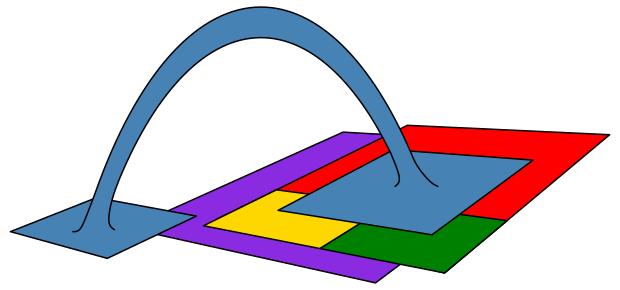
\includegraphics{bridge.png}
  \caption{A depiction of Peirce's Bridge for lines of identity}
  \footnotesize Source:\hspace{3pt}\url{https://commons.wikimedia.org/wiki/File:4CT_Inadequacy_Explanation.svg}
  \labfig{eg-bridge}
\end{marginfigure}

After introducing Selectives, Peirce further remarks on the next page:
\begin{quote}
  In order to avoid the intersection of Lines of Identity, either a Selective
may be employed, or a \emph{Bridge}, which is imagined to be a bit of paper
ribbon.
\end{quote}
This proposed alternative solution of having so-called \emph{Bridges} is quite
interesting, in that it makes the syntax of EG \emph{three-dimensional}, in
order to preserve the continuity of lines. A nice illustration of the bridge is
given in \reffig{eg-bridge}. We found this picture in the Wikipedia article on
the \emph{four color theorem} \cite{noauthor_four_2023}, which is no
coincidence: according to Burch \cite{sep-peirce}:
\begin{quote}
  Peirce began to research the four-color map conjecture, to work on the
graphical mathematics of de Morgan's associate A. B. Kempe, and to develop
extensive connections between logic, algebra, and topology, especially
topological graph theory. Ultimately these researches bore fruit in his
existential graphs [...]
\end{quote}

\paragraph{Multisets}

The Wikipedia article on Alfred Kempe also mentions the following interesting
fact \cite{noauthor_alfred_2023}:
\begin{quote}
  Kempe (1886) revealed a rather marked philosophical bent, and much influenced
Charles Sanders Peirce. Kempe also discovered what are now called multisets,
although this fact was not noted until long after his death.
\end{quote}
In fact, we can also give a multiset formalization of the syntax of graphs in
\sys{Beta}, based on the previous idea of replacing teridentities by variables.

\todo{Give the definition and some example}

\todo{What about the illative transformations?}